\chapter{A bibliometric study of research topics, collaboration and influence in
the field of the Iterated Prisoner's Dilemma}\label{chapter:bibliometric_study}

\begin{center}
    The research reported in this Chapter has lead to a manuscript, entitled: \\
    \textbf{``A bibliometric study of research topics, collaboration and influence in the field of the Iterated Prisoner's Dilemma''} \\
    Available at: \url{arxiv.org/abs/1911.06128} \\
    Associated data set: \cite{auction_data_2018}, \cite{anarchy_data_2018}, \cite{pd_data_2018}\\ \vspace{.5cm}
    The manuscript's abstract is the following:
\end{center}

This manuscript explores the research topics and collaborative behaviour of
authors in the field of the Prisoner's Dilemma using topic modelling and a graph
theoretic analysis of the co-authorship network. The analysis identified five
research topics in the Prisoner's Dilemma which have been relevant of the course
of time. These are human subject research, biological studies, strategies,
evolutionary dynamics on networks and modelling problems as a Prisoner's Dilemma
game. Moreover, the results demonstrated the Prisoner's Dilemma is a field of
continued interest, and although it is a collaborative field, it is not
necessarily more collaborative than other scientific fields. The co-authorship
network suggests that authors are focused on their communities and not many
connections across the communities are made. The Prisoner Dilemma authors also
do not influence or gain much information by their connections, unless they are
connected to a ``main'' group of authors.

The differences between the Chapter and the manuscript include \dots.   % TODO
\newpage

\section{Introduction}\label{section:introduction}

This Chapter presents a bibliometric analysis of the data set
``Articles' meta data on the Prisoner's Dilemma''~\cite{pd_data_2018}.
Chapter~\ref{chapter:literature_review} presented a review of published works on
the PD, and manually assigned them to different topics. To accompany that
manual identification of topics this Chapter presents an automatic approach
using natural language processing. More specifically, the \totalarticles articles' metadata
in~\cite{pd_data_2018} are used to extract a list of research topics in the field.
Moreover, the list of authors in~\cite{pd_data_2018} is also used to generate a
co-authorship network and explore their collaborative behaviour.
The Chapter is structured as follows:

\begin{itemize}
    \item section~\ref{section:methodology}, covers the data collection and an introduction
    to topic modelling and co-authorship networks.
    \item section~\ref{section:preliminary}, presents a preliminary analysis of the
    data set.
    \item section~\ref{section:topics}, identifies research topics in the field using
    natural language processing.
    \item section~\ref{section:co_authorship}, evaluates the collaborative behaviour
    of the field.
\end{itemize}

\section{Methodology}\label{section:methodology}

As discussed in~\cite{youngblood2018}, bibliometrics (the statistical analysis
of published works originally described by~\cite{pritchard1969}) has been used
to support historical assumptions about the development of fields
\cite{raina1998}, identify connections between scientific growth and policy
changes \cite{das2016}, develop a quantitative understanding of author
order~\cite{sekara2018}, and investigate the collaborative structure of an
interdisciplinary field~\cite{Liu2015}. Most academic research is undertaken in
the form of collaborative effort and as~\cite{Kyvik2017} points out, it is
rational that two or more people have the potential to do better as a group
than individually. Indeed this is the very premise of the PD itself.
Collaboration in groups has a long tradition in experimental
sciences and it has be proven to be productive according
to~\cite{Etzkowitz1992}. The number of collaborations can be different
between research fields and understanding how collaborative a field is not
always an easy task. Several studies tend to consider academic citations as a
measure for these things. A blog post published by Nature~\cite{nature_blog}
argues that depending on citations can often be misleading because the true
number of citations can not be known. Citations can be missed due to data entry
errors, academics are influenced by many more papers than they actually cite and
several of the citations are superficial.

A more recent approach to measuring collaborative behaviour, and to studying the
development of a field is to use the co-authorship network, as described
in~\cite{Liu2015}. The co-authorship network has many advantages as several
graph theoretic measures can be used as proxies to explain author relationships.
For example the average degree of a node corresponds to the average number of
an authors' collaborators, and clustering coefficient corresponds to the extent that
two collaborators of an author also collaborate with each other.
In~\cite{Liu2015}, the approach was applied to analyse the development of the field
``evolution of cooperation'', and in~\cite{youngblood2018} to identify the
subdisciplines of the interdisciplinary field of ``cultural evolution'' and
investigate trends in collaboration and productivity between these subdisciplines.
This Chapter builds on the works of~\cite{Liu2015} and ~\cite{youngblood2018} and
and extends their methodology. This is described in
section~\ref{section:co_authorship_network}.

Latent Dirichlet Allocation (LDA) is a topic modelling technique proposed
in~\cite{Blei2003} as a generative probabilistic model for discovering
underlying topics in collections of data.
Applications of the technique include detection in image data~\cite{Agarwal2008,
Coelho2010} and detection in video~\cite{Niebles2008, Wang2008}. Nevertheless,
LDA has been applied by several works on publication data for identifying the
topic structure of a subject area. In~\cite{Inglis2018}, it was applied to the
publications on mathematical education of the journals ``Educational Studies in
Mathematics'' and ``Journal for Research in Mathematics Education'', in~\cite{Sugimoto2011}
to the dissertations of the North American library and Information Science and
in~\cite{Bergmann2018} to conference papers presented at EvoLang conferences.
LDA is the topic modelling technique used in this thesis. An introduction to
the technique is presented in section~\ref{section:lda_introduction}.

Several of the approaches of this Chapter have previously been carried
out in~\cite{Bergmann2018,Liu2015,Sugimoto2011, youngblood2018}. The novelty of this
thesis is the combination of these approaches and their application to a new data
set. The data sets of~\cite{Liu2015} and~\cite{youngblood2018} are from 
from a single source, the Web of Science, whereas the data set~\cite{pd_data_2018}
considered here has been collected from five sources using a bespoke open source
software. This software and the data collection process are presented in
section~\ref{section:data_collection_arcas}.

\subsection{Data Collection}\label{section:data_collection_arcas}

Academic articles are accessible through scholarly databases. Several databases
and collections today offer access through an open application protocol
interface (API). An API allows users to query directly a journal's database and
bypass the graphical user interface. Interacting with an API has two phases:
requesting and receiving. The request phase includes composing a url with the
details of the request. For example,
\url{http://export.arxiv.org/api/query?search_query=abs:prisoner's
dilemma&max_results=1} represents a request message. The first part of the
request is the address of the API. In this example the address corresponds to
the API of arXiv. The second part of the request contains the search arguments.
In this example it is requested a single article that the word `prisoners dilemma' exists within
the article's title. The format of the request message is different from API to
API. The receive phase includes receiving a number of raw metadata of articles
that satisfies the request message. The raw metadata are commonly received in
extensive markup language (xml) or Javascript object notation (json)
formats~\cite{nurseitov2009}. Similarly to the request message, the structure of
the received data differs from journal
to journal.

The data collection is crucial to this thesis. To ensure that the research
reported in this Chapter can be reproduced all code used to query the different
APIs has been packaged as a Python library called \textit{Arcas}. The source
code of the library has been made available online and the package includes
documentation of usage which is available at:
\url{http://arcas.readthedocs.io/en/latest/}. Arcas allows users to communicate
with a list of APIs by specifying a single keyword whilst not considering the
differences between the requesting and receiving phases of the APIs. Consider
the example of retrieving a single article with the word `Prisoners Dilemma' in
the title. Figure~\ref{fig:arcas_query_plos} demonstrates the Python code needed
to query the publisher PLOS and Figure~\ref{fig:arcas_query_nature} demonstrates 
code for querying the API of Nature.

The only distinction between the two code snippets is their respective line 2
where the API is specified by creating an instance of a class corresponding
to the publisher's API. The differences between querying the two APIs are visible from
lines 6 and 12-onwards. Lines 6 show the requesting message and lines 12-onwards
show the metadata of the article received by each source.

\begin{figure}[!hbtp]
\begin{minted}
    [
    bgcolor=orange!25,
    framesep=2mm,
    frame=lines,
    baselinestretch=1.2,
    fontsize=\footnotesize,
    linenos
    ]
    {python}
>>> import arcas
>>> api = arcas.Plos()
>>> parameters = api.parameters_fix(title="Prisoner's Dilemma", records=1)
>>> url = api.create_url_search(parameters)
>>> url
http://api.plos.org/search?q=title:"Prisoner\'s Dilemma"&rows=1

>>> request = api.make_request(url)
>>> root = api.get_root(request)
>>> article = api.parse(root)
>>> article
[{'id': '10.1371/journal.pone.0028576',
'journal': 'PLoS ONE',
'eissn': '1932-6203',
'publication_date': '2011-12-14T00:00:00Z',
'article_type': 'Research Article',
'author_display': ['Irina Kareva'],
'abstract': ["As tumors outgrow their ..."],
'title_display': "Prisoner's Dilemma in Cancer Metabolism",
'score': 21,
'author': ['Irina Kareva'],
'date': 2011,
'provenance': 'PLOS',
'doi': '10.1371/journal.pone.0028576',
'url': 'https://doi.org/10.1371/journal.pone.0028576',
'title': "Prisoner's Dilemma in Cancer Metabolism",
'key': 'Kareva2011',
'unique_key': '0d56101113057d99fc6d83095812735a',
'category': 'Not available',
'open_access': 'Not available'}]
\end{minted}
\caption{Example of using the library Arcas to communicate the API of the publisher
PLOS. The query is for a single article with the word `prisoners dilemma' in
the title.}\label{fig:arcas_query_plos}
\end{figure}

\begin{figure}[!hbtp]
    \begin{minted}
        [
        bgcolor=orange!25,
        framesep=2mm,
        frame=lines,
        baselinestretch=1.2,
        fontsize=\footnotesize,
        linenos
        ]
        {python}
>>> import arcas
>>> api = arcas.Nature()
>>> parameters = api.parameters_fix(title="Prisoner's Dilemma", records=1)
>>> url = api.create_url_search(parameters)
>>> url
http://www.nature.com/opensearch/request?&query=dc.title adj Prisoner's Dilemma&maximumRecords=1

>>> request = api.make_request(url)
>>> root = api.get_root(request)
>>> article = api.parse(root)
>>> article
[{'records': None,
'record': None,
'recordSchema': 'info:srw/schema/11/pam-v2.1',
'recordPacking': 'packed',
'recordData': None,
'message': None,
'article': None,
'head': None,
'identifier': 'doi:10.1057/ces.1994.6',
'title': """Survey Article: Cooperate or Defect? Russian and American Students
in a Prisoner's Dilemma""",
'creator': 'Michael Hemesath',
'productCode': 'ces',
'publicationName': 'Comparative Economic Studies',
'issn': '0888-7233',
'eIssn': '1478-3320',
'doi': '10.1057/ces.1994.6',
'publisher': 'Palgrave Macmillan',
'publicationDate': '1994-04',
'volume': '36',
'number': '1',
'startingPage': '83',
'endingPage': '93',
'url': 'http://dx.doi.org/10.1057/ces.1994.6',
'genre': 'Research',
'description': "<p>Do assumptions underlying the models of ...",
'copyright': '© 1994 Palgrave Macmillan Ltd',
'aggregationType': 'issue'}]
    \end{minted}
    \caption{Example of using the library Arcas to communicate the API of the publisher
    Nature. The query is for a single article with the word `prisoners dilemma' in
    the title.}\label{fig:arcas_query_nature}
\end{figure}

There are differences and similarities between the retrievable metadata of each API. Arcas
includes a function which standarises the format of querying results. Figure~\ref{fig:arcas_to_dataframe}
demonstrates the usage of the function.

\begin{figure}[!hbtp]
    \begin{minted}
        [
        bgcolor=orange!25,
        framesep=2mm,
        frame=lines,
        baselinestretch=1.2,
        fontsize=\footnotesize,
        ]
        {python}
>>> meta_data = api.to_dataframe(article[0])
>>> meta_data.columns
Index(['url', 'key', 'unique_key', 'title', 'author', 'abstract', 'doi',
'date', 'journal', 'provenance', 'category', 'score', 'open_access'],
dtype='object')
\end{minted}
\caption{Python Code. Arcas includes a function which standarises the results of
the queries regarding the API.}\label{fig:arcas_to_dataframe}
\end{figure}

There are a total of five different APIs implemented within the project. These
five include APIs of four prominent publishers in the field and a preprint
server. Namely these are:

\begin{multicols}{2}
    \begin{itemize}
        \item arXiv~\cite{mckiernan2000}; a repository of electronic preprints.
        It consists of scientific
        papers in the fields of mathematics, physics, astronomy, electrical engineering,
        computer science, quantitative biology, statistics, and quantitative finance,
        which all can be accessed online.
        \item PLOS~\cite{plos}; a library of open access journals and other scientific literature
        under an open content license. It launched its first journal, PLOS Biology,
        in October 2003 and publishes seven journals, as of October 2015.
        \item IEEE Xplore Digital Library (IEEE)~\cite{ieee}; a research database for discovery
        and access to journal articles, conference proceedings, technical standards,
        and related materials on computer science, electrical engineering and electronics,
        and allied fields. It contains material published mainly by the Institute of
        Electrical and Electronics Engineers and other partner publishers. 
        \item Nature~\cite{nature}; a multidisciplinary scientific journal,
        first published on 4 November 1869. It was ranked the world's most cited
        scientific journal by the Science Edition of the 2010 Journal Citation Reports
        and is ascribed an impact factor of 40.137, making it one of the world's
        top academic journals.
        \item Springer~\cite{springer}; a leading global scientific publisher of
        books and journals. It publishes close to 500 academic and professional
        society journals.
    \end{itemize}
\end{multicols}

Each APIs has a corresponding class implemented in Arcas. The classes include
a series of methods which allow Arcas to communicate with the APIs. A example
of an API class is given by both Figure~\ref{fig:arcas_arxiv} and Figure~\ref{fig:arcas_ieee}.
These include the classes for the APIs of arXiv and IEEE. Note that IEEE is
an example of an API which requires a user to have an access key
(line 7 in Figure~\ref{fig:arcas_ieee}). An access key can be required from the
publishers website and for the APIs of this work they can acquired for free.

\begin{figure}[!hbtp]
    \begin{minted}
        [
        bgcolor=orange!5,
        framesep=2mm,
        frame=lines,
        baselinestretch=1.2,
        fontsize=\scriptsize,
        linenos
        ]
        {python}
class Arxiv(Api):
    def __init__(self):
        self.standard = 'http://export.arxiv.org/api/query?search_query='

    def to_dataframe(self, raw_article):
        """A function which takes a dictionary with structure of the arXiv results,
        transforms it to a standardized format and returns a dataframe."""
        raw_article['url'] = raw_article.get('id', None)

        for key_one, key_two in [['author', 'name'], ['category', 'category']]:
            raw_article[key_one] = raw_article.get(key_two, None)
            if raw_article[key_one] is not None:
                raw_article[key_one] = raw_article[key_one].split(',')

        raw_article['abstract'] = raw_article.get('summary', None)
        raw_article['date'] = int(raw_article.get('published', '0').split('-')[0])
        raw_article['journal'] = raw_article.get('journal_ref', None)
        if raw_article['journal'] is None:
            raw_article['journal'] = "arXiv"

        raw_article['provenance'] = 'arXiv'
        raw_article['title'] = raw_article.get('title', None)
        raw_article['doi'] = raw_article.get('doi', None)
        raw_article['key'], raw_article['unique_key'] = self.create_keys(raw_article)

        raw_article['open_access'] = True
        raw_article['score'] = 'Not available'
        return self.dict_to_dataframe(raw_article)

    def parse(self, root):
        """Removing unwanted branches."""
        branches = root.getchildren()
        raw_articles = []
        for record in branches:
            if 'entry' in record.tag:
                raw_articles.append(self.xml_to_dict(record))
        if not raw_articles:
            raw_articles = False
        return raw_articles

    @staticmethod
    def parameters_fix(author=None, title=None, abstract=None, year=None, records=None,
                       start=None, category=None, journal=None, keyword=None):
        parameters = []
        if author is not None:
            parameters.append('au:{}'.format(author))
        if title is not None:
            parameters.append('ti:{}'.format(title))
        if abstract is not None:
            parameters.append('abs:{}'.format(abstract))
        if category is not None:
            parameters.append('cat:{}'.format(category))
        if journal is not None:
            parameters.append('jr:{}'.format(journal))
        if keyword is not None:
            parameters.append('all:{}'.format(keyword))
        if records is not None:
            parameters.append('max_results={}'.format(records))
        if start is not None:
            parameters.append('start={}'.format(start))
        if year is not None:
            print('ArXiv does not support argument year.')

        return parameters

    @staticmethod
    def get_root(response):
        root = ElementTree.fromstring(response.text)
        return root
\end{minted}
\caption{Class Arxiv is implemented in Arcas. It includes the code necessary for Arcas
to query the API of arXiv.}\label{fig:arcas_arxiv}
\end{figure}

\begin{figure}[!hbtp]
    \begin{minted}
        [
        bgcolor=orange!5,
        framesep=2mm,
        frame=lines,
        baselinestretch=1.2,
        fontsize=\scriptsize,
        linenos
        ]
        {python}
class Ieee(Api):
    """
        API argument is 'ieee'.
    """
    def __init__(self):
        self.standard = 'https://ieeexploreapi.ieee.org/api/v1/search/articles?'
        self.key_api = api_key

    def create_url_search(self, parameters):
        """Creates the search url, combining the standard url and various
        search parameters."""
        url = self.standard
        url += parameters[0]
        for i in parameters[1:]:
            url += '&{}'.format(i)
        url += '&apikey={}'.format(self.key_api)
        return url

    @staticmethod
    @ratelimit.rate_limited(3)
    def make_request(url):
        """Request from an API and returns response."""
        response = requests.get(url, stream=True, verify=False)
        if response.status_code != 200:
            raise APIError(response.status_code)
        return response

    def parse(self, root):
        """Parsing the xml file"""
        if root['total_records'] == 0:
            return False
        return root['articles']

    @staticmethod
    def parameters_fix(author=None, title=None, abstract=None, year=None,
                        records=None, start=None, category=None, journal=None,
                        keyword=None):
        parameters = []
        if author is not None:
            parameters.append('author={}'.format(author))
        if title is not None:
            parameters.append('article_title={}'.format(title))
        if abstract is not None:
            parameters.append('abstract={}'.format(abstract))
        if year is not None:
            parameters.append('publication_year={}'.format(year))
        if category is not None:
            parameters.append('index_terms={}'.format(category))
        if journal is not None:
            parameters.append('publication_title={}'.format(journal))
        if keyword is not None:
            parameters.append('querytext={}'.format(keyword))
        if records is not None:
            parameters.append('max_records={}'.format(records))
        if start is not None:
            parameters.append('start_record={}'.format(start))

        return parameters

    @staticmethod
    def get_root(response):
        root = response.json()
        return root
    
\end{minted}
\caption{Class Ieee is implemented in Arcas. It includes the code necessary for Arcas
to query the API of IEEE.}\label{fig:arcas_ieee}
\end{figure}

As mentioned in Chapter~\ref{chapter:introduction} the source code associated
with the research projects of this thesis have been written following a set of
best practices. These best practices include unit testing. There are a series of
unit tests that test the functionality and correctness of each API class.
For example, Figure~\ref{fig:test_arxiv} displays a test case for the
method \mintinline{python}{to_dataframe} of the class Arxiv. Moreover, Figure
\ref{fig:test_ieee} shows several unit tests which ensure that the requesting
url for IEEE, with different search arguments, is being generated correctly.

\begin{figure}[!hbtp]
    \begin{minted}
        [
        bgcolor=orange!5,
        framesep=2mm,
        frame=lines,
        baselinestretch=1.2,
        fontsize=\scriptsize,
        linenos
        ]
        {python}
import arcas

def test_to_dataframe():
    dummy_article = {'entry': '\n', 'id': 'http://arxiv.org/abs/0000',
                     'updated': '2011', 'published': '2010', 'title': 'Title',
                     'summary': "Abstract", 'author': '\n', 'name': 'E Glynatsi, V Knight',
                     'doi': '10.0000', 'comment': 'This is a comment.',
                     'journal_ref': 'Awesome Journal', 'primary_category': 'Dummy',
                     'category': None}
    api = arcas.Arxiv()
    article = api.to_dataframe(dummy_article)

    assert isinstance(article, pandas.core.frame.DataFrame)
    assert list(article.columns) == api.keys()
    assert len(article['url']) == 2

    assert article['url'].unique()[0] == 'http://arxiv.org/abs/0000'
    assert article['key'].unique()[0] == 'Glynatsi2010'
    assert article['title'].unique()[0] == 'Title'
    assert article['abstract'].unique()[0] == 'Abstract'
    assert article['journal'].unique()[0] == 'Awesome Journal'
    assert article['primary_category'].unique()[0] == 'Dummy'
    assert article['category'].unique()[0] == None
    assert article['score'].unique()[0] == 'Not available'
    assert article['open_access'].unique()[0] == True
\end{minted}
\caption{Unit tests for class Arxiv. Tests the functionality of the method \mintinline{python}{to_dataframe}.}\label{fig:test_arxiv}
\end{figure}

\begin{figure}[!hbtp]
        \begin{minted}
            [
            bgcolor=orange!5,
            framesep=2mm,
            frame=lines,
            baselinestretch=1.2,
            fontsize=\scriptsize,
            linenos
            ]
            {python}
import arcas

def test_setup():
    api = arcas.Ieee()
    assert api.standard == 'https://ieeexploreapi.ieee.org/api/v1/search/articles?'

def test_parameters_and_url_author():
    api = arcas.Ieee()
    parameters = api.parameters_fix(author='Glynatsi')
    assert parameters == ['author=Glynatsi']

    url = api.create_url_search(parameters)
    assert url == 'https://ieeexploreapi.ieee.org/api/v1/search/articles?author=Glynatsi&apikey=Your key here'

def test_parameters_and_url_title():
    api = arcas.Ieee()
    parameters = api.parameters_fix(title='Game')
    assert parameters == ['article_title=Game']

    url = api.create_url_search(parameters)
    assert url == 'https://ieeexploreapi.ieee.org/api/v1/search/articles?article_title=Game&apikey=Your key here'
\end{minted}
\caption{Unit tests for class Ieee.}\label{fig:test_ieee}
\end{figure}


The \totalarticles articles metadata~\cite{pd_data_2018} explored in this Chapter has been collected
using Arcas. More specifically, articles for which any of the terms
``prisoner's dilemma'', ``prisoners dilemma'', ``prisoner dilemma'', ``prisoners
evolution'', ``prisoner game theory'' existed within the title, the abstract or
the text are included in the analysis. The data set has been archived and is
available at~\cite{pd_data_2018}. Note that the latest data collection was
performed on the \(30^{\text{th}}\) November 2018.

\subsection{Co-authorship Network}\label{section:co_authorship_network}

The relationship between the authors within a field will be modelled as a graph
\(G = (V_G, E_G)\) where \(V_G\) is the set of nodes and \(E_G\)  is the set of
edges. The set \(V_G\) represents the authors and an edge connects two authors
if and only if those authors have written together. This co-authorship network is
constructed using the data set~\cite{pd_data_2018} and the open source package
\cite{networkx}. The PD network is denoted as \(G\) where the
number of unique authors \(|V(G)|\) is \authors and \(|E(G)|\) is \edges.
All authors' names were formatted as their first name and last name (i.e.
Martin A. Nowak to Martin Nowak). This was done to avoid errors such as Martin
A. Nowak and Martin Nowak being treated as a different person. There are some
authors for which only their first initial was found. These entries are left as
such.

The collaborativeness of the authors will be analysed using measures such as, isolated nodes,
connected components, clustering coefficient, communities, modularity and average degree.
These measures show the number of connections authors can have
and how strongly connected these people are. The number of isolated nodes is the
number of nodes that are not connected to another node, thus the
number of authors that have published alone. The average degree denotes the average
number of neighbours for each nodes, i.e. the average number of collaborations
between the authors.
A connected component is a maximal set of nodes such that each pair of nodes is
connected by a path~\cite{Easley2010}. The number of connected components as well as the size of the
largest connected component in the network are reported.
The size of the largest connected component represents the scale of the central cluster
of the entire network, as will be discussed in later parts.
Clustering coefficient and modularity are also calculated. The clustering
coefficient, defined as 3 times the number of triangles on the graph divided
by the number of connected triples of nodes, is a local measure of the degree to
which nodes in a graph tend to cluster together
in a clique~\cite{Easley2010}. It shows to which extent the collaborators
of an author also write together.

In comparison, modularity is a global measure designed to measure the strength of
division of a network into communities. The number of communities will be reported
using the Clauset-Newman-Moore method~\cite{clauset2004}. Also the modularity index
is calculated using the Louvain method described in~\cite{Blondel2008}. The value
of the modularity index can vary between \([-1, 1]\), a high value of modularity
corresponds to a structure where there are dense connections between the nodes within
communities but sparse connections between nodes in different communities.
That means that there are many sub communities of authors that write together
but not across communities.

Two further points are aimed to be explored in this thesis, (1) which people control the flow
of information;
as in which people influence the field the most and (2) which are the authors that
gain the most from the influence of the field. To measure these concepts
centrality measures are going to be used.
Centrality measures are often used to understand different
aspects of social networks~\cite{Landherr2010}. The two centrality measures chosen
here are closeness and betweenness centrality.

\begin{enumerate}
    \item In networks some nodes have a short distance to a lot of nodes and
    consequently are able to spread information on the network very effectively.
    A representative of this idea is \textbf{closeness centrality}, where a node
    is seen as centrally involved in the network if it requires only few
    intermediaries to contact others and thus is structurally relatively
    independent. Closeness centrality is interpreted as influence. Authors with a high
    value of closeness centrality, are the authors that spread scientific
    knowledge easier on the network and they have high influence.
    \item Another centrality measure is the \textbf{betweenness centrality},
    where the determination of an author's centrality is based on the quotient
    of the number of all shortest paths between nodes in the network that
    include the node in question and the number of all shortest paths in the
    network. In betweenness centrality the position of the node matters. Nodes
    with a higher value of betweenness centrality are located in positions that
    a lot of information pass through, this is interpreted as the gain from
    the influence, thus these authors gain the most from their networks.
\end{enumerate}

\subsection{Topic Modelling}\label{section:lda_introduction}

The articles contained in the data set will be classified
into research topics using LDA, a topic modelling technique
designed to summarize large collections of documents by a small number of
conceptually connected topics or themes~\cite{Blei2003, Grimmer2013}. LDA is
carried out using~\cite{rehurek_lrec}.

The input to an LDA is a collection of documents, and the collection of
documents considered here are the articles' abstracts. The output of an LDA is
an \(N \times n\) matrix - \(N\) rows for \(N\) abstracts and \(n\) columns for
\(n\) topics. The cells contain the percentage contributions for each topic for
each abstract, \(c_i^ j\) for \(i \in \{1, 2, \dots, n\}\) for \(j \in \{1, 2,
\dots, N\}\). Thus each document/abstract is represented by a distribution over
topics, and the topics themselves are represented by a distribution over words.
More specifically, each topics is described by weights associated with words.
For example assume two topics A and B were the words and their associated weights
are:

\begin{itemize}
    \item Topic A: \(0.039 \times\)``cooperation'', \(0.028 \times\)``study'' and \(0.026 \times\)``human''.
    \item Topic B: \(0.020 \times\)``cooperation'', \(0.028 \times\)``agents'' and
    \(0.026 \times\)``strategies''.
\end{itemize}

The percentage contribution for a document with abstract ``The study of
cooperation in humans'' has a \(c_{A} = 0.039 + 0.028 + 0.026 = 0.093\) and
\(c_B = .020 + 0.0 + 0.0 = 0.020\). In essence, LDA maps every paper to a
vector. In this example the document is mapped to \([0.093, 0.020]\). Each
document has a dominant topic to which is going to be assigned in. The dominant
topic is the topic with the highest percentage contribution denoted as \(c^*\).
For the given example the dominant topic is Topic A \(c^*=c_A\).

LAD requires that the number of topics is specified in advance before running
the algorithm. The number of topics can be chosen using the coherence
value~\cite{Roder2015} or through subjective minimisation of the overlapping
keywords between two topics. Both these approaches will be used in this work.
Preceding the analysis of research topics, the next the next section presents a
preliminary analysis of the data set.

\section{Preliminary Analysis}\label{section:preliminary}

The data set~\cite{pd_data_2018} consists of \totalarticles articles with unique
titles. In case of duplicates the preprint version of an article (collected from
arXiv) was dropped. Similarly to~\cite{Liu2015}, \manual articles have been manually
added throughout the writing of Chapter~\ref{chapter:literature_review} because
they were of specific interest. These papers include~\cite{Flood1958} the first
publication on the PD,~\cite{Ohtsuki2006, Stewart2012} two well cited
articles in the field, and a series of works from Robert Axelrod
~\cite{Axelrod1980a, Axelrod1980b, Axelrod1987, Axelrod1981, Riolo2001}.

A more detailed summary of the articles' provenance
is given by Table~\ref{table:preliminary_table}. Only 3\% of the data set consists of
articles that were manually added and 27\% of the articles were collected from
arXiv. The average number of publications is also included in
Table~\ref{table:preliminary_table}. Overall an average of 43 articles are published
per year on the topic. The most significant contribution to this appears to be
from arXiv with 11 articles per year, followed by Springer with 9 and PLOS with
8.

\begin{table}[!hbtp]
    \begin{center}
    \resizebox{.9\textwidth}{!}{
    \begin{tabular}{lrrrr}
\toprule
{} &  Number of Articles &  Percentage \% &  Year of first publication &  Average number of publications per year\\
\midrule
IEEE     &               294 &       12.14\% &                    1973 &                             5\\
Manual   &                76 &        3.14\% &                    1951 &                             1\\
Nature   &               436 &       18.00\% &                    1959 &                             8\\
PLOS     &               477 &       19.69\% &                    2005 &                             8\\
Springer &               533 &       22.01\% &                    1966 &                             9\\
arXiv    &               654 &       27.00\% &                    1993 &                            11\\
Overall  &              2470 &      100.00\% &                    1951 &                            43\\
\bottomrule
\end{tabular}
}
    \end{center}
    \caption{Summary of~\cite{pd_data_2018} per provenance.}
    \label{table:preliminary_table}
\end{table}

The data handled  here is in fact a time series from the 1950s, the formulation
of the game, until 2018 (Figure~\ref{fig:timeseries}). Two observations can be
made from Figure~\ref{fig:timeseries}.

\begin{enumerate}
    \item There is a steady increase of the number of publications since the
    1980s and the introduction of computer tournaments~\cite{Axelrod1981}.
    \item There is a decrease in 2017-2018. This is due to our data set being
    incomplete. Articles that have been written in 2017-2018 have either not
    being published or were not retrievable by the APIs at the time of the last
    data collection.
\end{enumerate}

These observations can be confirmed by studying the time series.
Using~\cite{scipy}, an exponential distribution is fitted to the data.
The fitted model can be used to forecast the
behaviour of the field for the next 5 years. Even
though the time series has indicated a slight decrease, the model forecasts that
the number of publications will keep increasing, thus demonstrating that the
field of the PD continues to attract academic attention.

\begin{figure}[!hbtp]
    \centering
    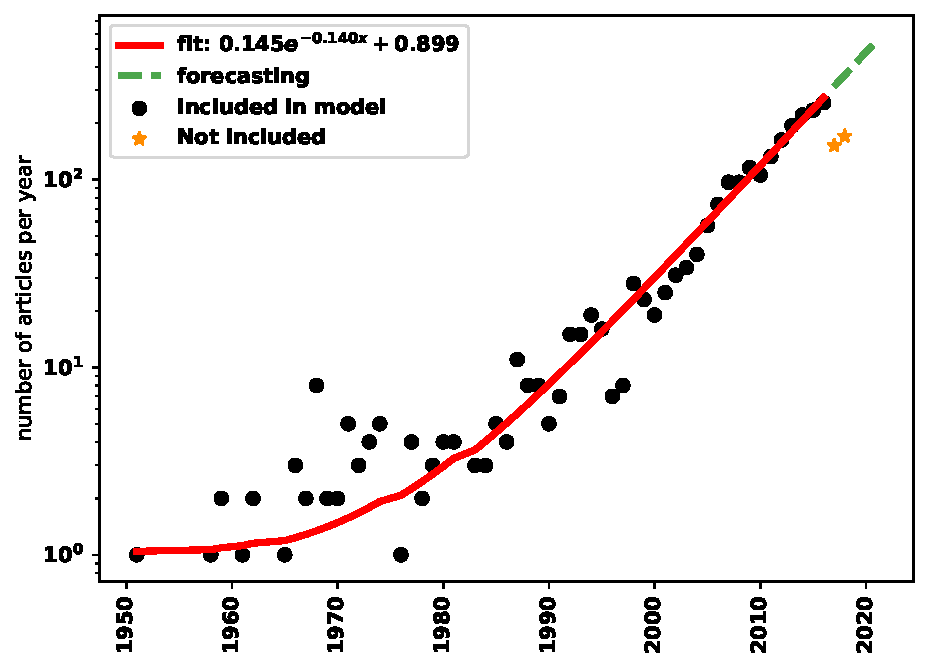
\includegraphics[width=.50\textwidth]{src/chapters/03/paper/bibliometric-study-of-the-prisoners-dilemma/assets/images/forecasting.pdf}
    \caption{Number of articles published on the PD 1951-2018 (on a log scale),
    with a fitted exponential line, and a forecast for 2017-2022.}\label{fig:timeseries}
\end{figure}

There are a total of \authors authors in the data set and several of these
authors have had multiple publications collected from the data collection process.
The highest number of articles collected for an
author is 83 publications for Matjaz Perc. The distribution of the number of
papers per author is given by Figure~\ref{fig:num_papers_per_author}, and it can
be seen that Matjaz Perc is an outlier. More specifically, most authors have
1 to 6 publications in the data set.

\begin{figure}[!hbtp]
    \centering
    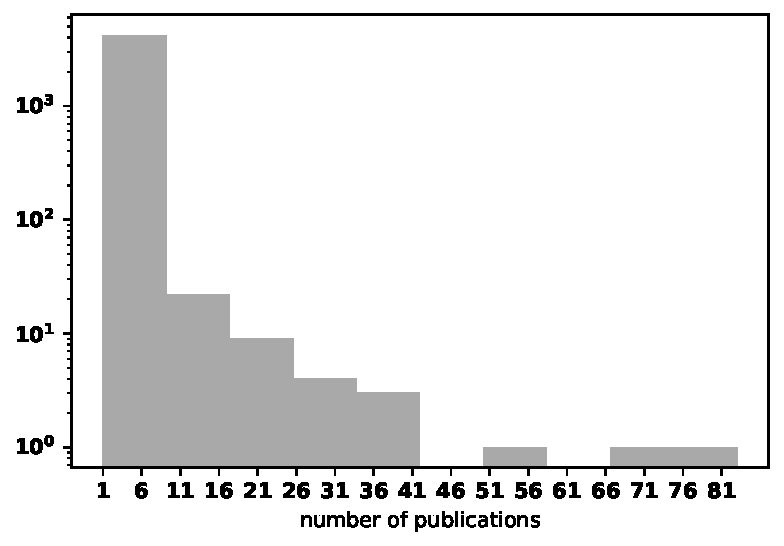
\includegraphics[width=.50\textwidth]{src/chapters/03/paper/bibliometric-study-of-the-prisoners-dilemma/assets/images/papers_per_author.pdf}
    \caption{Distribution of number of papers per author (on a log scale).}
    \label{fig:num_papers_per_author}
\end{figure}

The overall Collaboration Index (CI) or the average number of authors on
multi-authored papers is 3.2, thus on average a non single author publication in
the PD has 3 authors. This appears to be quite standard compared to other fields
such as cultural evolution~\cite{youngblood2018}, Astronomy and Astrophysics,
Genetics and Heredity, Nuclear and Particle Physics as reported
by~\cite{nature_author_blog}.
There are only a total of 545 publications with a single author, which
corresponds to the 22\% of the papers. It appears that academic publications
tend to be undertaken in the form of collaborative effort, which is in line
with the claim of~\cite{Kyvik2017}. From
Figure~\ref{fig:ci_over_time} the trend of CI over the years is given. There are
some peaks in the early years 1969 and 1980, however, a steady increase appears
to happen after 2004. This could be an effect of better communication tools
being introduced around that time which enabled more collaborations between
researchers.

\begin{figure}[!hbtp]
    \centering
    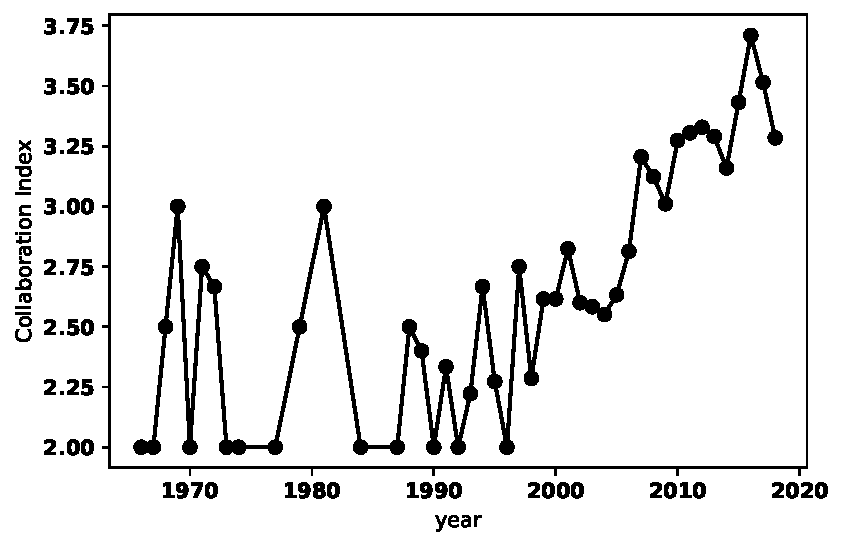
\includegraphics[width=.55\textwidth]{src/chapters/03/paper/bibliometric-study-of-the-prisoners-dilemma/assets/images/collaborative_index.pdf}
    \caption{Collaboration index over time.}\label{fig:ci_over_time}
\end{figure}

The collaborativeness of the authors is explored in more detail in
Section~\ref{section:co_authorship} using the co-authorship network. The
collaborative behaviour and relative influence of authors will also be explored
in co-authorship networks which correspond to their publications research topics.
These topics are presented in the next section.

\section{Research topics in the Prisoner's Dilemma research}\label{section:topics}

In order to identify the topics which are being discussed in the field of the
PD, the LDA algorithm implemented in~\cite{rehurek_lrec} is applied to the
abstracts of the data set. As mentioned before, the number of topics, which
will be denoted as \(n\), needs to be specified before running the algorithm.
The appropriate number of topics is chosen based on the coherence
value~\cite{Roder2015}. Figure~\ref{fig:coherence_value_over_number_of_topcis}
gives the coherence values of 18 models where \(n \in \{2, 3, \dots, 19\}\), and
it can be seen than the most appropriate number of topics is 6 with a coherence
value of 0.418.

\begin{figure}[!hbtp]
    \centering
    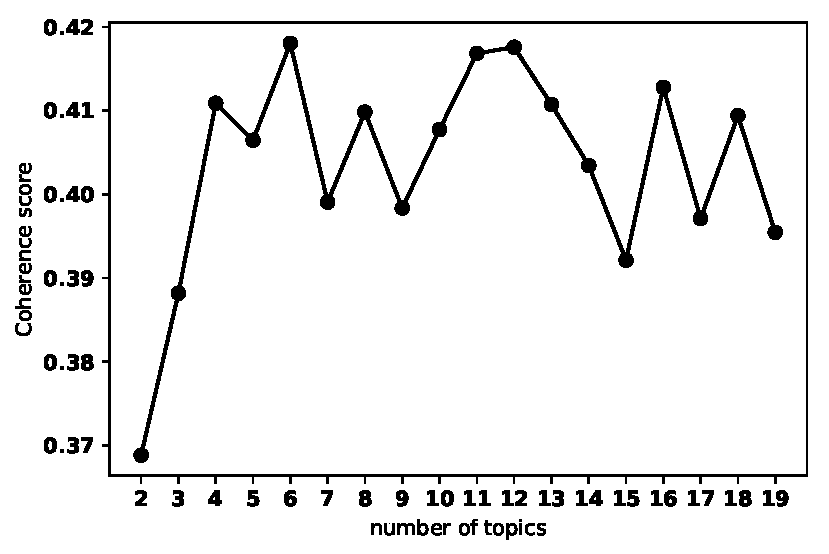
\includegraphics[width=.45\textwidth]{src/chapters/03/paper/bibliometric-study-of-the-prisoners-dilemma/assets/images/coherence_values.pdf}
    \caption{Coherence for LDA models over the number of topics.}
    \label{fig:coherence_value_over_number_of_topcis}
\end{figure}

The keywords associated with each topic for \(n=6\) are given by
Table~\ref{table:topics_keywords_n_6}. Though \(n=6\) has the highest coherence
score, from Table~\ref{table:topics_keywords_n_6} it can be observed that there
are overlapping keywords between the topics. Further manual investigation has
revealed that the seperation of topics are the most clear when an \(n\) of \(5\)
is considered. The LDA model for \(n=5\) has a coherence value 0.406 which is
close to 0.418 (the score for \(n=6\). Thus, \(n=5\) is chosen to carry out the analysis of this work.


\begin{table}[!hbtp]
    \begin{center}
    \resizebox{\textwidth}{!}{
    \begin{tabular}{lc}
\toprule
Topic & Topic Keywords \\
\midrule
A &                     model, theory, system, base, paper, problem, propose, present, approach, provide, analysis, framework, method, develop, solution \\
B &          \textcolor{red}{behavior}, \textcolor{red}{social}, human, decision, study, experiment, make, suggest, result, behaviour, effect, partner, participant, subject, experimental \\
C &                         individual, group, good, \textcolor{red}{social}, punishment, level, cost, mechanism, dilemma, cooperative, show, base, public, high, society \\
D &                          game, strategy, player, agent, play, dilemma, state, prisoner, payoff, equilibrium, result, iterate, set, probability, show \\
E &         population, evolutionary, dynamic, model, selection, result, evolution, evolve, show, process, size, \textcolor{red}{interaction}, \textcolor{red}{cooperator}, change, system \\
F &  cooperation, network, \textcolor{red}{interaction}, structure, study, evolution, find, \textcolor{red}{behavior}, cooperative, simulation, rule, spatial, \textcolor{red}{cooperator}, promote, result \\
\bottomrule
\end{tabular}
}
    \end{center}
    \caption{Keywords for each topic when \(n=6\). The highlighted keywords are overlapping keywords between topics.}
    \label{table:topics_keywords_n_6}
\end{table}

For \(n=5\) the articles are clustered and assigned to their dominant topic,
based on the highest percentage contribution. The keywords associated with a
topic, the most representative article of the topic (based on the
percentage contribution) and its academic reference are given by
Table~\ref{table:topics_and_articles}. The topics are labelled as A, B, C, D and
E, and more specifically:

\begin{itemize}
    \item Based on the keywords associated with Topic A, and the most
    representative article, Topic A appears to be about \textbf{human subject
    research}. Several publications assigned to the topic study the PD by
    setting experiments and having human participants simulate the game
    instead of computer simulations. These articles include~\cite{Matsumoto2016}
    which showed that prosocial behaviour increased with the age of the
    participants,~\cite{Li20140} which studied the difference in cooperation
    between high-functioning autistic and typically developing
    children,~\cite{Molina2013} explored the gender effect in highschool
    students and~\cite{Bell2017} explored the effect of facial expressions of
    individuals.
    \item Though it is not immediate from the keywords associated with
    Topic B, investigating the papers assigned to the topic indicate that it
    is focused on \textbf{biological studies}. Papers assigned to the topic include
    papers which apply the PD to genetics~\cite{Santorelli2008, Sistrom2015}, to
    the study of tumours~\cite{archetti2013evolutionary, sartakhti2017} and
    viruses~\cite{turner1999prisoner}. Other works include how phenotype affinity
    can affect the emergence of cooperation~\cite{wu2019phenotype} and modelling
    bacterial communities as a spatial structured social dilemma.
    \item Based on the keywords and the most representative article Topic
    C appears to include publications on PD \textbf{strategies}. Publications
    in the topic include the introduction of new strategies~\cite{stewart2013extortion},
    the search of optimality in strategies~\cite{banerjee2007reaching} and the
    training of strategies~\cite{ishibuchi2011evolution} with different
    representation methods. Moreover, publications that study the evolutionary
    stability of strategies~\cite{Adami2013} and introduced methods
    of differentiating between them~\cite{Ashlock2008} are
    also assigned to C.
    \item The keywords associated with Topic D clearly show that the topic
    is focused on \textbf{evolutionary dynamics on networks}. Publications include
    \cite{ichinose2013robustness} which explored the robustness of cooperation
    on networks,~\cite{wang2012spatial} which studied the effect of a strategy's neighbourhood
    on the emergence of cooperation and~\cite{chen2016fixation} which explored
    the fixation probabilities of any two strategies is spatial
    structures.
    \item The publication assigned to Topic E are on \textbf{modelling problems
    as a PD game}. Though Topic B is also concerned with problems being formulated
    as a PD, it includes only biological problems. In comparison, the problems
    in Topic E include decision making in
    operational research~\cite{ormerod2010or}, information sharing among members
    in a virtual team~\cite{feng2008trilateral}, the measurement of influence
    in articles based on citations~\cite{hutchins2016relative} and the price
    spikes in electric power markets~\cite{Guan2002}, and not on biological studies.
\end{itemize}

\begin{table}[!hbtp]
    \begin{center}
    \resizebox{\textwidth}{!}{
    \begin{tabularx}{1.5\textwidth}{lXXl|cc}
\toprule
Dominant Topic &                                                                                                 Topic Keywords &                                                                                                                                    Most Representative Article Title &        Reference &  \# Documents &  \% Documents \\
\midrule
A &                 social, behavior, human, study, experiment, cooperative, cooperation, suggest, find, behaviour &                                                                                      Facing Aggression: Cues Differ for Female versus Male Faces &  \cite{Geniole2012} &                496.0 &                   0.2008 \\
B &                               individual, group, good, show, high, increase, punishment, cost, result, benefit &  Genomic and Gene-Expression Comparisons among Phage-Resistant Type-IV Pilus Mutants of Pseudomonas syringae pathovar phaseolicola &  \cite{Sistrom2015} &                309.0 &                   0.1251 \\
C &                             game, strategy, player, agent, dilemma, play, payoff, state, prisoner, equilibrium &                                                            Fingerprinting: Visualization and Automatic Analysis of Prisoner's Dilemma Strategies &  \cite{Sistrom2015} &                561.0 &                   0.2271 \\
D &  cooperation, network, population, evolutionary, evolution, interaction, dynamic, structure, cooperator, study &                                                   Influence of initial distributions on robust cooperation in evolutionary  Prisoner's Dilemma &     \cite{Chen2007} &                556.0 &                   0.2251 \\
E &                           model, theory, base, system, problem, paper, propose, information, provide, approach &                                                                          Gaming and price spikes in electric power markets and possible remedies &     \cite{Guan2002} &                548.0 &                   0.2219 \\
\bottomrule
\end{tabularx}
}
    \end{center}
    \caption{Keywords for each topic and the document with the most representative article for each topic.}
    \label{table:topics_and_articles}
\end{table}

Note that the whilst for the choice of 5 topics the actual clustering is not
subjective (the algorithm is determining the output) the interpretation above is.

Thus, the five topics in the PD publications identified by the data set of using an LDA
are:

 \begin{enumerate} 
    \item human subject research, 
    \item biological studies, 
    \item strategies, 
    \item evolutionary dynamics on networks, 
    \item modelling problems as a PD.
\end{enumerate}
These topics nicely
summarise the PD research. They highlight the interdisciplinarity of the field;
how it brings together applied modelling of real world situations (Topic B and E)
and more theoretical notions such as evolutionary dynamics and optimality of
strategies.

Figure~\ref{fig:number_of_articles_per_topic} gives the number of articles
per topic over time. The topics appear to have had a similar trend over the years,
with topics B and D having a later start. Following the introduction of a topic
the publications in that topic have been increasing. There is no decreasing
trend in any of the topics. All the topics have been publishing for years and
they still attract the interest of academics. Thus, there does not
seem to be any given topic more or less in fashion.

\begin{figure}[!hbtp]
    \centering
    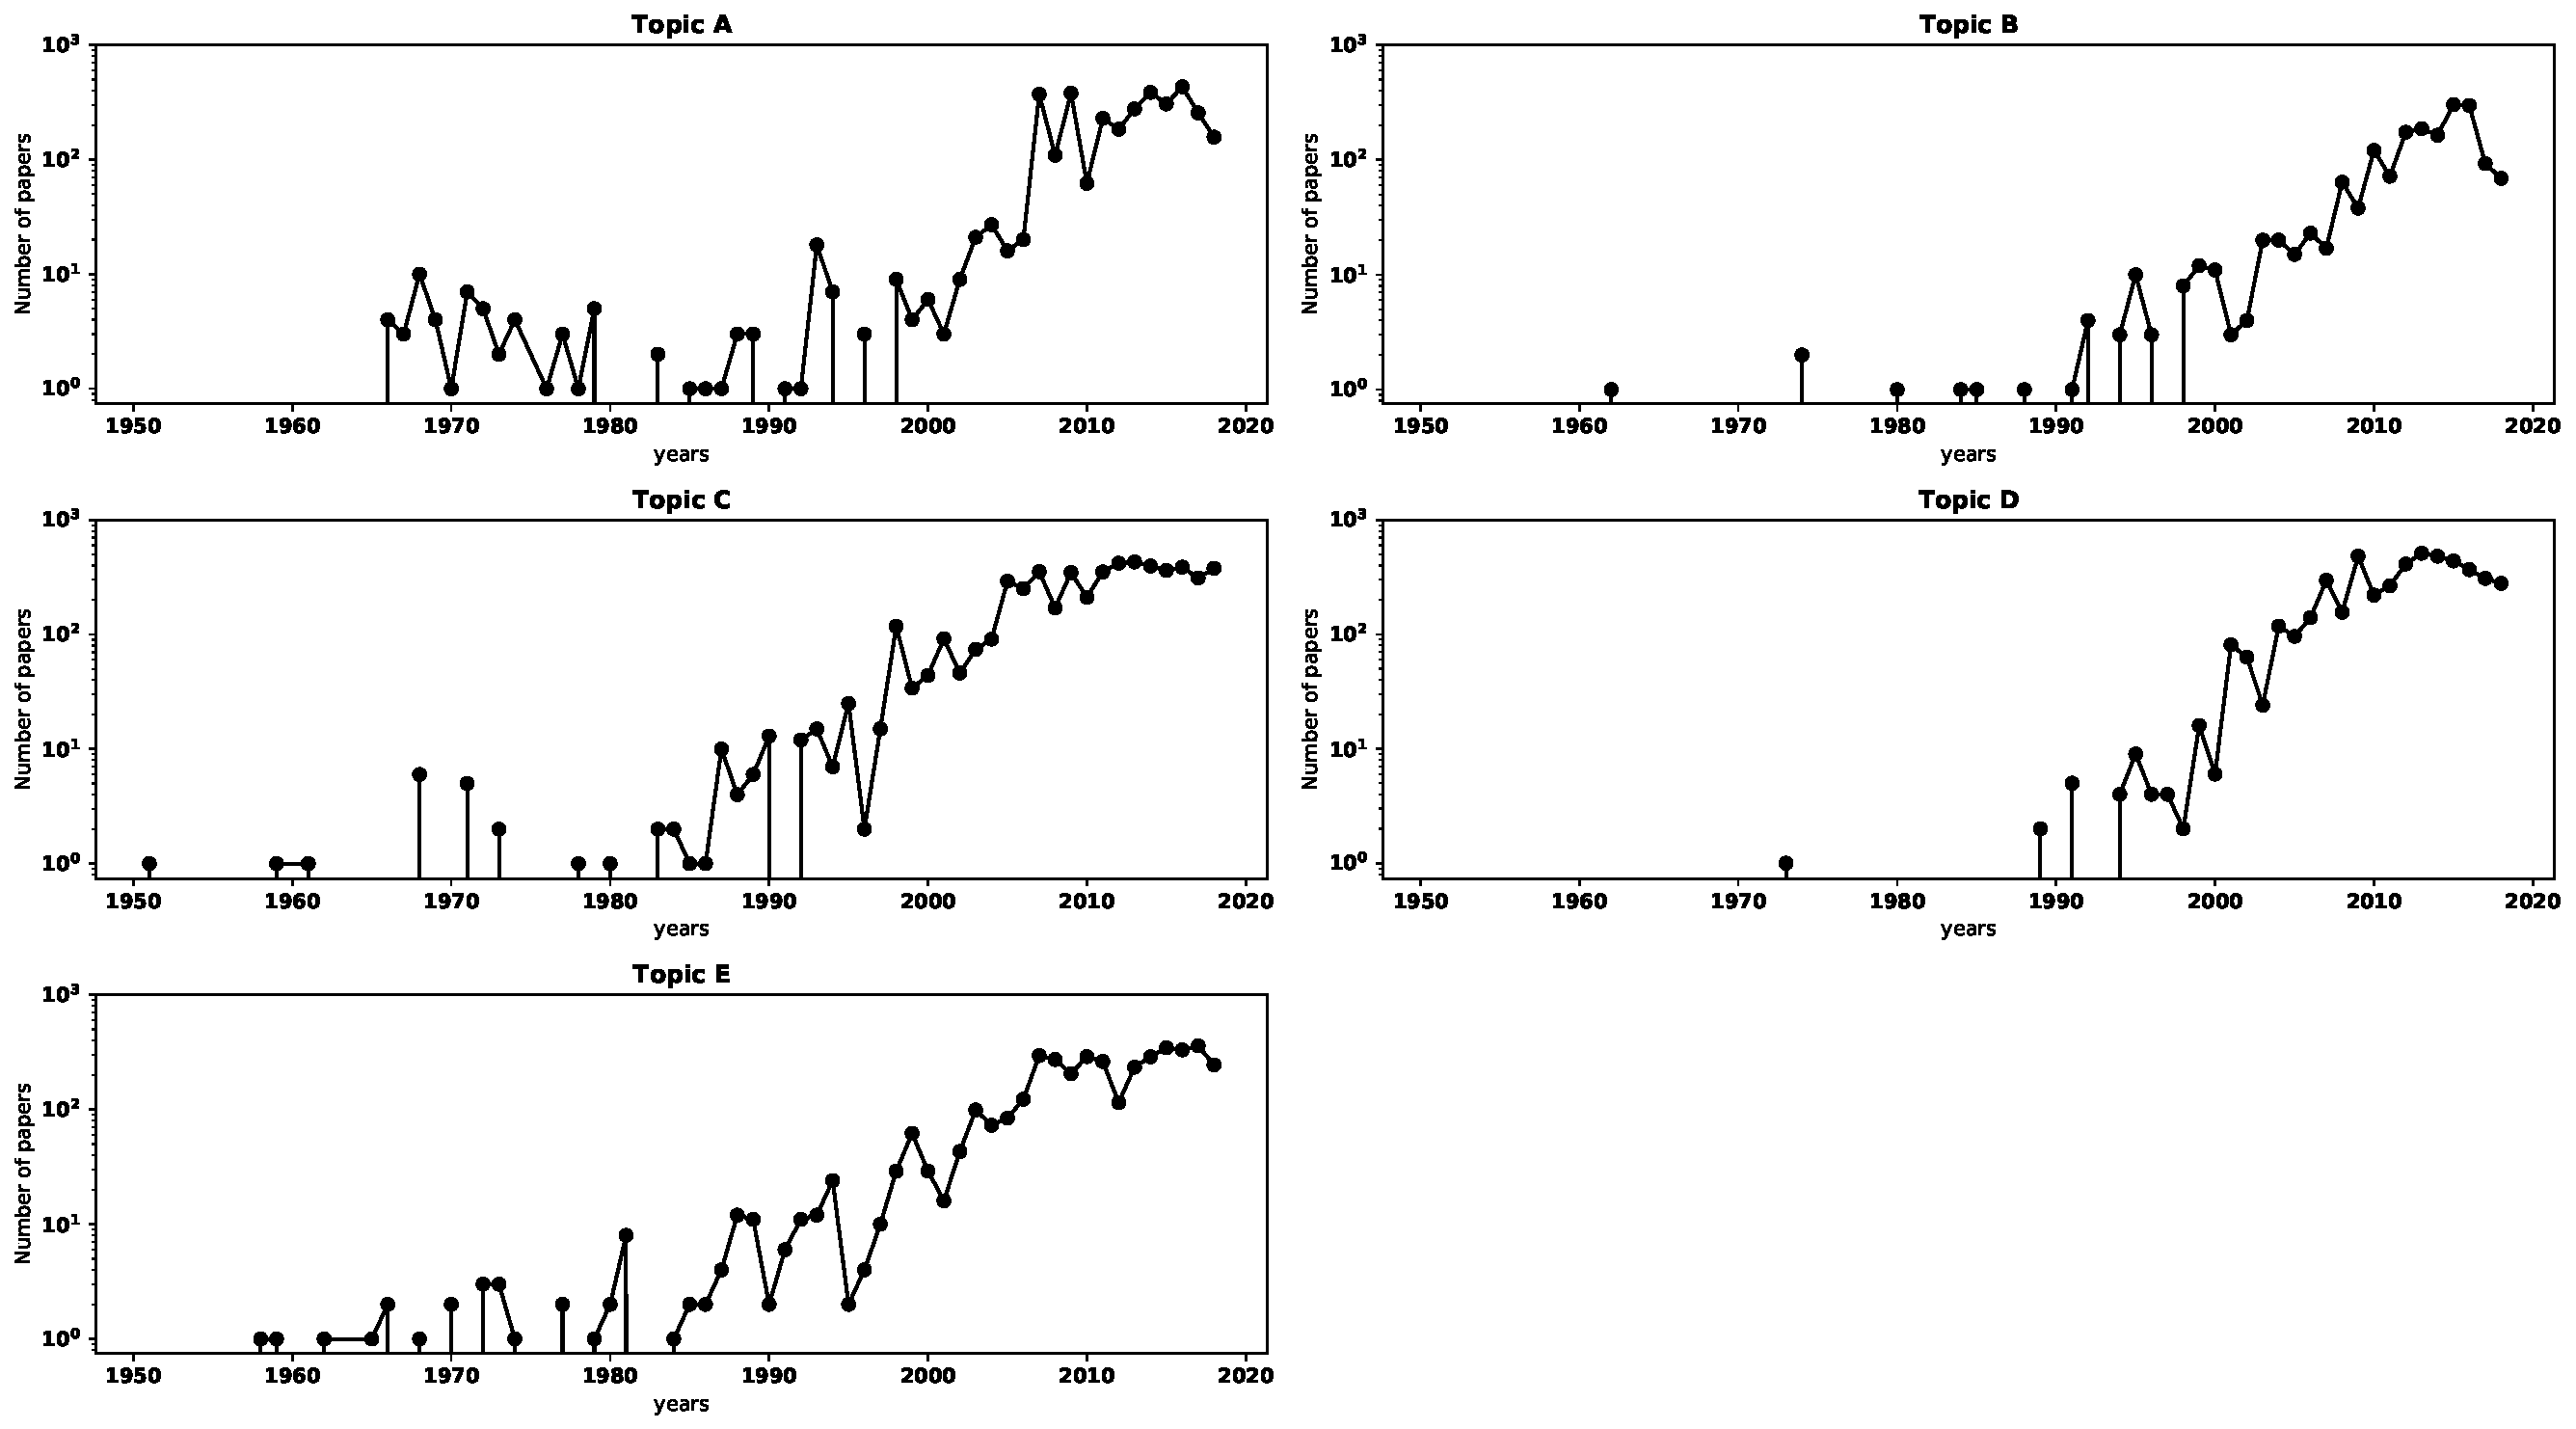
\includegraphics[width=\textwidth]{src/chapters/03/paper/bibliometric-study-of-the-prisoners-dilemma/assets/images/papers_per_topic_over_time.pdf}
    \caption{Number of articles per topic over the years (on a logged scale).}\label{fig:number_of_articles_per_topic}
\end{figure}

To gain a better understanding regarding the change in the topics over the years,
LDA is applied to the cumulative data set over 8 time periods. These periods are
1951-1965, 1951-1973, 1951-1980, 1951-1988, 1951-1995, 1951-2003, 1951-2010,
1951-2018. The number of topics for each cumulative subset is chosen based on
the coherence value and no objective approach is used. As a result, the period
1951-2018 has been assigned \(n=6\) which had the highest coherence
value instead of 5. The chosen models for each period including the
number of topics, their keywords and number of articles assigned to them are
given by Table \ref{table:topics_per_year}.

\begin{table}[!hbtp]
    \begin{center}
    \resizebox{\textwidth}{!}{
    \begin{tabular}{llccc}
\toprule
    Period &  Topic &                                                                                                Topic Keywords & Num of Documents & Percentage of Documents \\
\midrule
 1951-1965 &               1 &                 problem, technology, divert, euler, subsystem, requirement, trace, technique, system, untried &                3 &                   0.375 \\
 1951-1965 &               2 &            interpret, requirement, programme, evolution, article, increase, policy, system, trace, technology &                2 &                    0.25 \\
 1951-1965 &               3 &          equipment, agency, conjecture, development, untried, programme, trend, technology, weapon, technique &                1 &                   0.125 \\
 1951-1965 &               4 &                 variation, celebrated, trend, untried, change, involve, month, technique, subsystem, research &                1 &                   0.125 \\
 1951-1965 &               5 &                           give, good, modern, trace, technique, ambiguity, problem, trend, technology, system &                1 &                   0.125 \\
 \midrule
 1951-1973 &               1 &                           study, shock, cooperative, money, part, vary, investigate, good, receive, equipment &               12 &                  0.3243 \\
 1951-1973 &               2 &          cooperation, level, significantly, sequence, reward, provoke, descriptive, principal, display, argue &                4 &                  0.1081 \\
 1951-1973 &               3 &               player, make, effect, triad, experimental, motivation, dominate, hypothesis, instruction, trend &                3 &                  0.0811 \\
 1951-1973 &               4 &                                           ss, sex, male, female, dyad, design, suggest, college, factor, tend &                3 &                  0.0811 \\
 1951-1973 &               5 &               result, research, format, change, operational, analysis, relate, understanding, decision, money &                2 &                  0.0541 \\
 1951-1973 &               6 &                          condition, give, high, treatment, conflict, cc, real, original, replication, promote &                2 &                  0.0541 \\
 1951-1973 &               7 &              group, competitive, show, interpret, scale, compete, escalation, free, variable, individualistic &                2 &                  0.0541 \\
 1951-1973 &               8 &                        outcome, strategy, choice, type, pdg, difference, dummy, conclude, compare, consistent &                2 &                  0.0541 \\
 1951-1973 &               9 &                   game, difference, pair, approach, behavior, person, weapon, occur, advantaged, differential &                2 &                  0.0541 \\
 1951-1973 &              10 &                    response, present, dilemma, influence, cooperate, bias, point, amount, participate, factor &                2 &                  0.0541 \\
 1951-1973 &              11 &                       trial, problem, previous, involve, prisoner, experiment, follow, tit, increase, initial &                1 &                   0.027 \\
 1951-1973 &              12 &                           matrix, behavior, rational, black, model, research, broad, distance, complex, trace &                1 &                   0.027 \\
 1951-1973 &              13 &                    play, finding, individual, noncooperative, white, nature, race, ratio, represent, prisoner &                1 &                   0.027 \\
 \midrule
 1951-1980 &               1 &                                      play, trial, group, follow, white, interpret, scale, black, trend, small &               14 &                    0.25 \\
 1951-1980 &               2 &                              outcome, level, effect, type, dyad, vary, pdg, participate, understanding, arise &                9 &                  0.1607 \\
 1951-1980 &               3 &         game, strategy, cooperation, significant, difference, sentence, text, occur, differential, hypothesis &                4 &                  0.0714 \\
 1951-1980 &               4 &                        male, female, find, result, sex, subject, experimental, situation, treatment, computer &                4 &                  0.0714 \\
 1951-1980 &               5 &                         research, problem, influence, matrix, format, model, analysis, year, crime, equipment &                4 &                  0.0714 \\
 1951-1980 &               6 &                                    condition, dilemma, bias, free, attempt, book, year, dummy, prison, design &                4 &                  0.0714 \\
 1951-1980 &               7 &                    variable, result, factor, individual, ability, triad, half, migration, change, investigate &                3 &                  0.0536 \\
 1951-1980 &               8 &                 show, present, suggest, rational, compete, approach, characteristic, examine, person, conduct &                3 &                  0.0536 \\
 1951-1980 &               9 &                         behavior, high, finding, relate, obtain, assistance, ratio, good, weapon, competition &                3 &                  0.0536 \\
 1951-1980 &              10 &                               ss, shock, money, competitive, part, difference, pair, amount, man, information &                3 &                  0.0536 \\
 1951-1980 &              11 &             player, conflict, theory, decision, determine, produce, maker, cooperate, specialist, programming &                2 &                  0.0357 \\
 1951-1980 &              12 &            study, prisoner, make, response, experiment, noncooperative, standard, separate, conclude, initial &                2 &                  0.0357 \\
 1951-1980 &              13 &                       give, cooperative, choice, cognitive, real, operational, set, subject, ascribe, concern &                1 &                  0.0179 \\
 \midrule
 1951-1988 &               1 &                     trial, difference, find, choice, significant, competitive, effect, triad, interact, occur &               24 &                  0.2553 \\
 1951-1988 &               2 &                                            ss, shock, money, pair, response, part, high, tit, receive, amount &               13 &                  0.1383 \\
 1951-1988 &               3 &                         suggest, paper, case, debate, view, achieve, framework, natural, assumption, finitely &               10 &                  0.1064 \\
 1951-1988 &               4 &                     prisoner, dilemma, behavior, model, present, involve, person, increase, trust, experiment &                8 &                  0.0851 \\
 1951-1988 &               5 &                                   game, player, show, approach, repeat, previous, move, tat, related, include &                8 &                  0.0851 \\
 1951-1988 &               6 &                cooperation, level, mutual, equilibrium, standard, provide, information, human, real, question &                6 &                  0.0638 \\
 1951-1988 &               7 &                      play, result, male, subject, female, cooperative, sex, experimental, treatment, computer &                5 &                  0.0532 \\
 1951-1988 &               8 &                        research, study, variable, ability, factor, conflict, matrix, year, student, interpret &                4 &                  0.0426 \\
 1951-1988 &               9 &                                         problem, group, small, scale, social, issue, large, base, bias, party &                4 &                  0.0426 \\
 1951-1988 &              10 &                          game, strategy, outcome, type, cooperate, ethical, pdg, explain, dependent, separate &                4 &                  0.0426 \\
 1951-1988 &              11 &              give, condition, individual, major, dyad, behaviour, produce, conflict, assistance, collectively &                3 &                  0.0319 \\
 1951-1988 &              12 &                        situation, iterate, statement, rational, card, side, paradox, true, consequence, front &                2 &                  0.0213 \\
 1951-1988 &              13 &                               inflation, hypothesis, rate, run, change, demand, nominal, cost, output, growth &                2 &                  0.0213 \\
 1951-1988 &              14 &                                     theory, make, analysis, decision, system, examine, work, soft, lead, hard &                1 &                  0.0106 \\
 \midrule
 1951-1995 &               1 &                            strategy, population, evolution, iterate, tit, opponent, evolve, dynamic, set, tat &               31 &                  0.1732 \\
 1951-1995 &               2 &                 game, repeat, assumption, rule, person, equilibrium, general, finitely, indefinitely, analyze &               24 &                  0.1341 \\
 1951-1995 &               3 &                            inflation, long, rate, hypothesis, run, policy, cost, nominal, demand, programming &               20 &                  0.1117 \\
 1951-1995 &               4 &            condition, outcome, trial, find, difference, cooperation, experiment, level, significant, response &               15 &                  0.0838 \\
 1951-1995 &               5 &                     rational, result, receive, statement, money, paradox, shock, iterate, consequence, common &               14 &                  0.0782 \\
 1951-1995 &               6 &             cooperation, show, competitive, high, probability, conflict, simulation, altruism, yield, natural &               14 &                  0.0782 \\
 1951-1995 &               7 &                           prisoner, dilemma, give, point, defect, form, cooperator, increase, relate, ethical &               10 &                  0.0559 \\
 1951-1995 &               8 &                       player, give, decision, provide, cooperative, game, previous, pair, determine, interact &                9 &                  0.0503 \\
 1951-1995 &               9 &                          play, cooperate, result, male, subject, female, time, relationship, suggest, student &                8 &                  0.0447 \\
 1951-1995 &              10 &                                   problem, group, theory, good, approach, society, large, scale, issue, level &                8 &                  0.0447 \\
 1951-1995 &              11 &            study, situation, behaviour, computer, argue, change, implication, characteristic, real, associate &                8 &                  0.0447 \\
 1951-1995 &              12 &                        model, paper, behavior, examine, present, mutual, expectation, develop, type, variable &                7 &                  0.0391 \\
 1951-1995 &              13 &                                   make, research, system, analysis, choice, work, base, relation, world, wide &                6 &                  0.0335 \\
 1951-1995 &              14 &               individual, social, behavior, standard, choose, evolutionary, partner, payoff, defection, small &                5 &                  0.0279 \\
 \midrule
 1951-2003 &               1 &                                    game, player, dilemma, prisoner, theory, give, paper, make, group, problem &              151 &                  0.4266 \\
 1951-2003 &               2 &                         cooperation, result, play, show, cooperate, condition, cooperative, high, level, time &              106 &                  0.2994 \\
 1951-2003 &               3 &                  strategy, model, agent, study, behavior, individual, population, evolutionary, state, player &               97 &                   0.274 \\
 \midrule
 1951-2010 &               1 &                                  model, theory, paper, base, make, present, problem, provide, human, decision &              325 &                  0.3454 \\
 1951-2010 &               2 &                                   game, strategy, player, agent, play, dilemma, system, behavior, show, state &              322 &                  0.3422 \\
 1951-2010 &               3 &  cooperation, network, study, population, individual, evolutionary, social, evolution, interaction, structure &              294 &                  0.3124 \\
 \midrule
 1951-2018 &               1 &                              model, theory, system, base, paper, problem, propose, present, approach, provide &              556 &                  0.2251 \\
 1951-2018 &               2 &                        behavior, social, human, decision, study, experiment, make, suggest, result, behaviour &              482 &                  0.1951 \\
 1951-2018 &               3 &                     individual, group, good, social, punishment, level, cost, mechanism, dilemma, cooperative &              428 &                  0.1733 \\
 1951-2018 &               4 &                            game, strategy, player, agent, play, dilemma, state, prisoner, payoff, equilibrium &              380 &                  0.1538 \\
 1951-2018 &               5 &                 population, evolutionary, dynamic, model, selection, result, evolution, evolve, show, process &              351 &                  0.1421 \\
 1951-2018 &               6 &       cooperation, network, interaction, structure, study, evolution, find, behavior, cooperative, simulation &              273 &                  0.1105 \\
\bottomrule
\end{tabular}
}
    \end{center}
    \caption{Topic modelling result for the cumulative data set over the periods
    }\label{table:topics_per_year}
\end{table}

But how well do the five topics which were presented earlier fit the
publications over time? This is answered by comparing the performance of three
LDA models over the cumulative periods' publications. The three models are LDA
models for the entire data set for \(n\) equal to 5, 6 and the optimal number of topics over time. For
each model the \(c^*\) is estimated for each document in the cumulative data
sets. The performance of the models are then compared based on:

\begin{equation}\label{eq:ratio}
    \bar{c^*} \times n
\end{equation}

where \(\bar{c^*}\) is the median highest percentage contribution and \(n\)
is the number of topics of a given period. A model with more topics will have more
difficulty to assign papers. Thus, equation (ref{eq:ratio}) is a measure of confidence
in assigning a given paper to its topic weighted by the number of topics.
The performances are
given by Figure~\ref{fig:median_percentage_contribution_over_time}.

The five topics of the PD presented in this manuscript appear to always be
less good at fitting the publications compared to the six topics of LDA \(n=6\).
Moreover, there are less good than the topics of the optimal number of topics
from 1951 to 1995. The difference in the performance values, equation (\ref{eq:ratio}),
however are small. The relevances of the five topics has been increasing
over time, and though, the topics did not always fit the majority of published
work over time, there were still papers being published on those topics.

\begin{figure}[!hbtp]
    \centering
    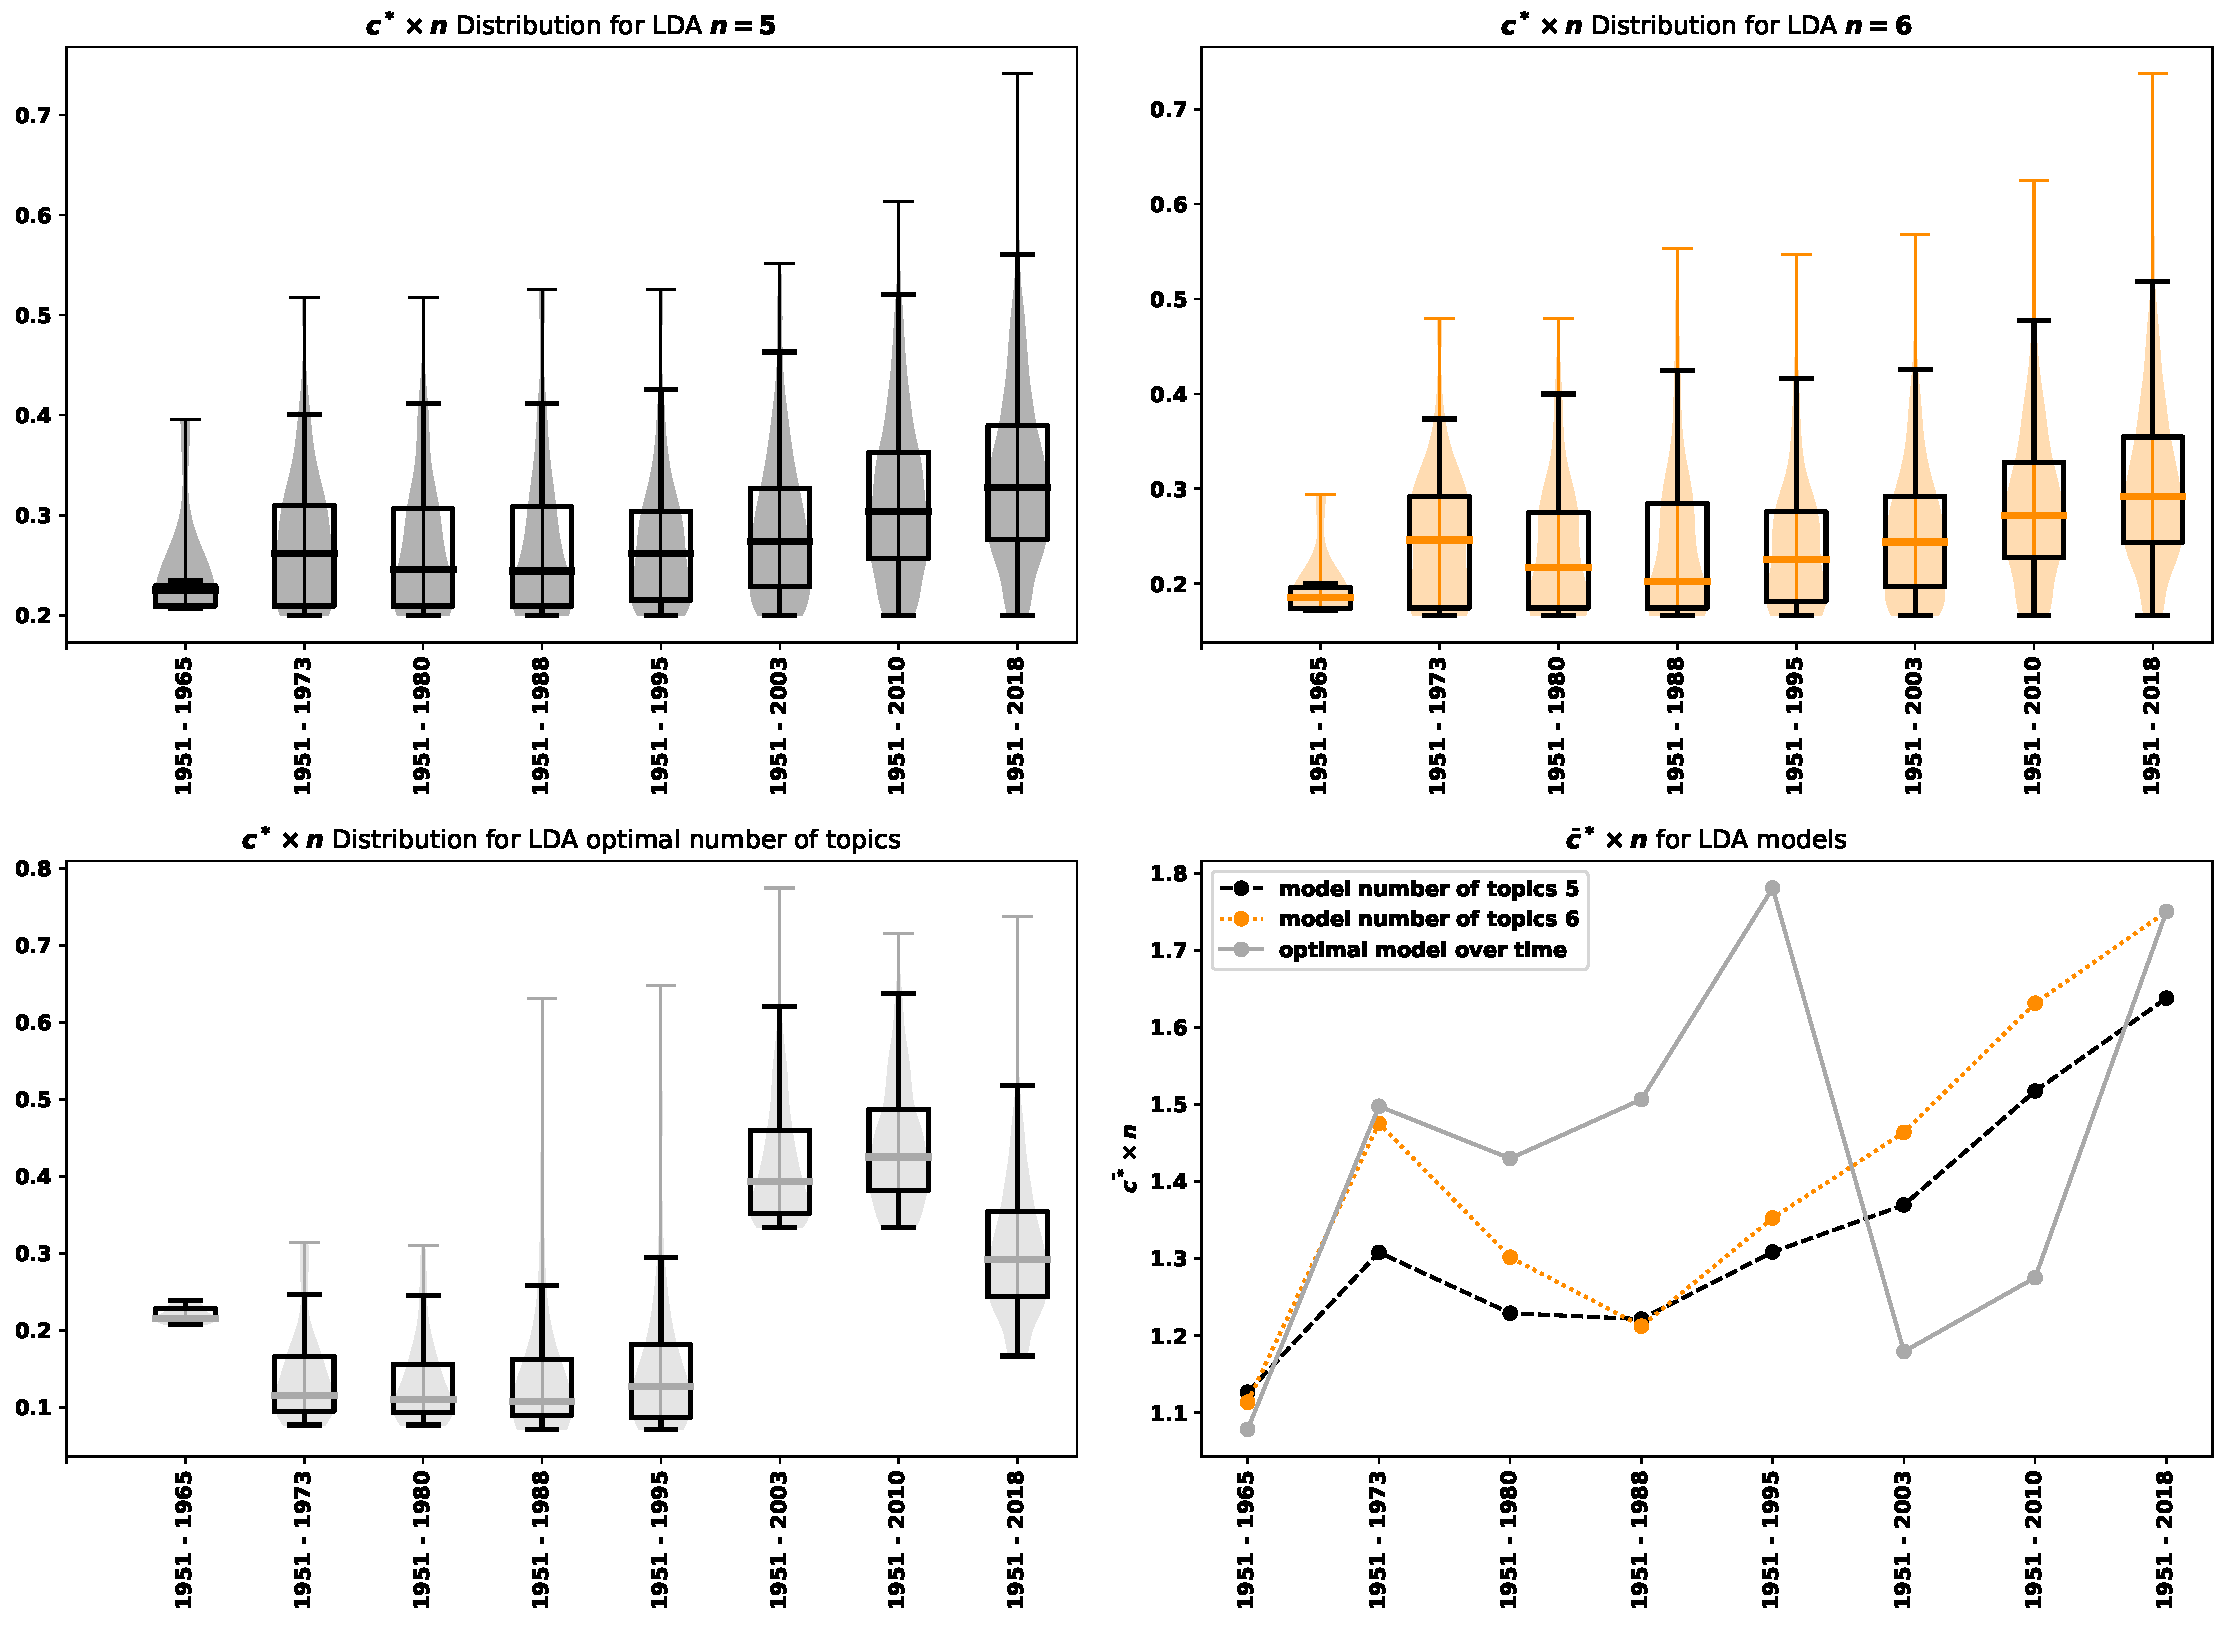
\includegraphics[width=.75\textwidth]{src/chapters/03/paper/bibliometric-study-of-the-prisoners-dilemma/assets/images/contribution_over_time.pdf}
    \caption{Maximum percentage contributions (\(c^*\)) over the time periods,
    for the LDA models for the entire data set for \(n\) equal to 5, 6
    and the optimal number of topics over time.}
    \label{fig:median_percentage_contribution_over_time}
\end{figure}

In the following section the collaborative behaviour of authors in the field,
and within the field's topics as were presented in this section, are explored
using a network theoretic approach.

\section{Analysis of co-authorship network}\label{section:co_authorship}

The collaborative behaviour of authors in the field of the PD is assessed using
the co-authorship network, which as introduced in
section~\ref{section:methodology} is denoted as \(G\). There are a total of
\connectedcomponents connected components in \(G\) and the largest component has
a size of \largestcc nodes. The largest connected component is going to be
refereed to as the main cluster of the network and is denoted as \(\bar{G}\). A
graphical representation of both networks is shown in
Figures~\ref{fig:graphical_representation_g}-\ref{fig:graphical_representation_g_bar}
and a metrics summary is given by Table~\ref{table:network_comparison.tex}.

\begin{figure}[!hbtp]
    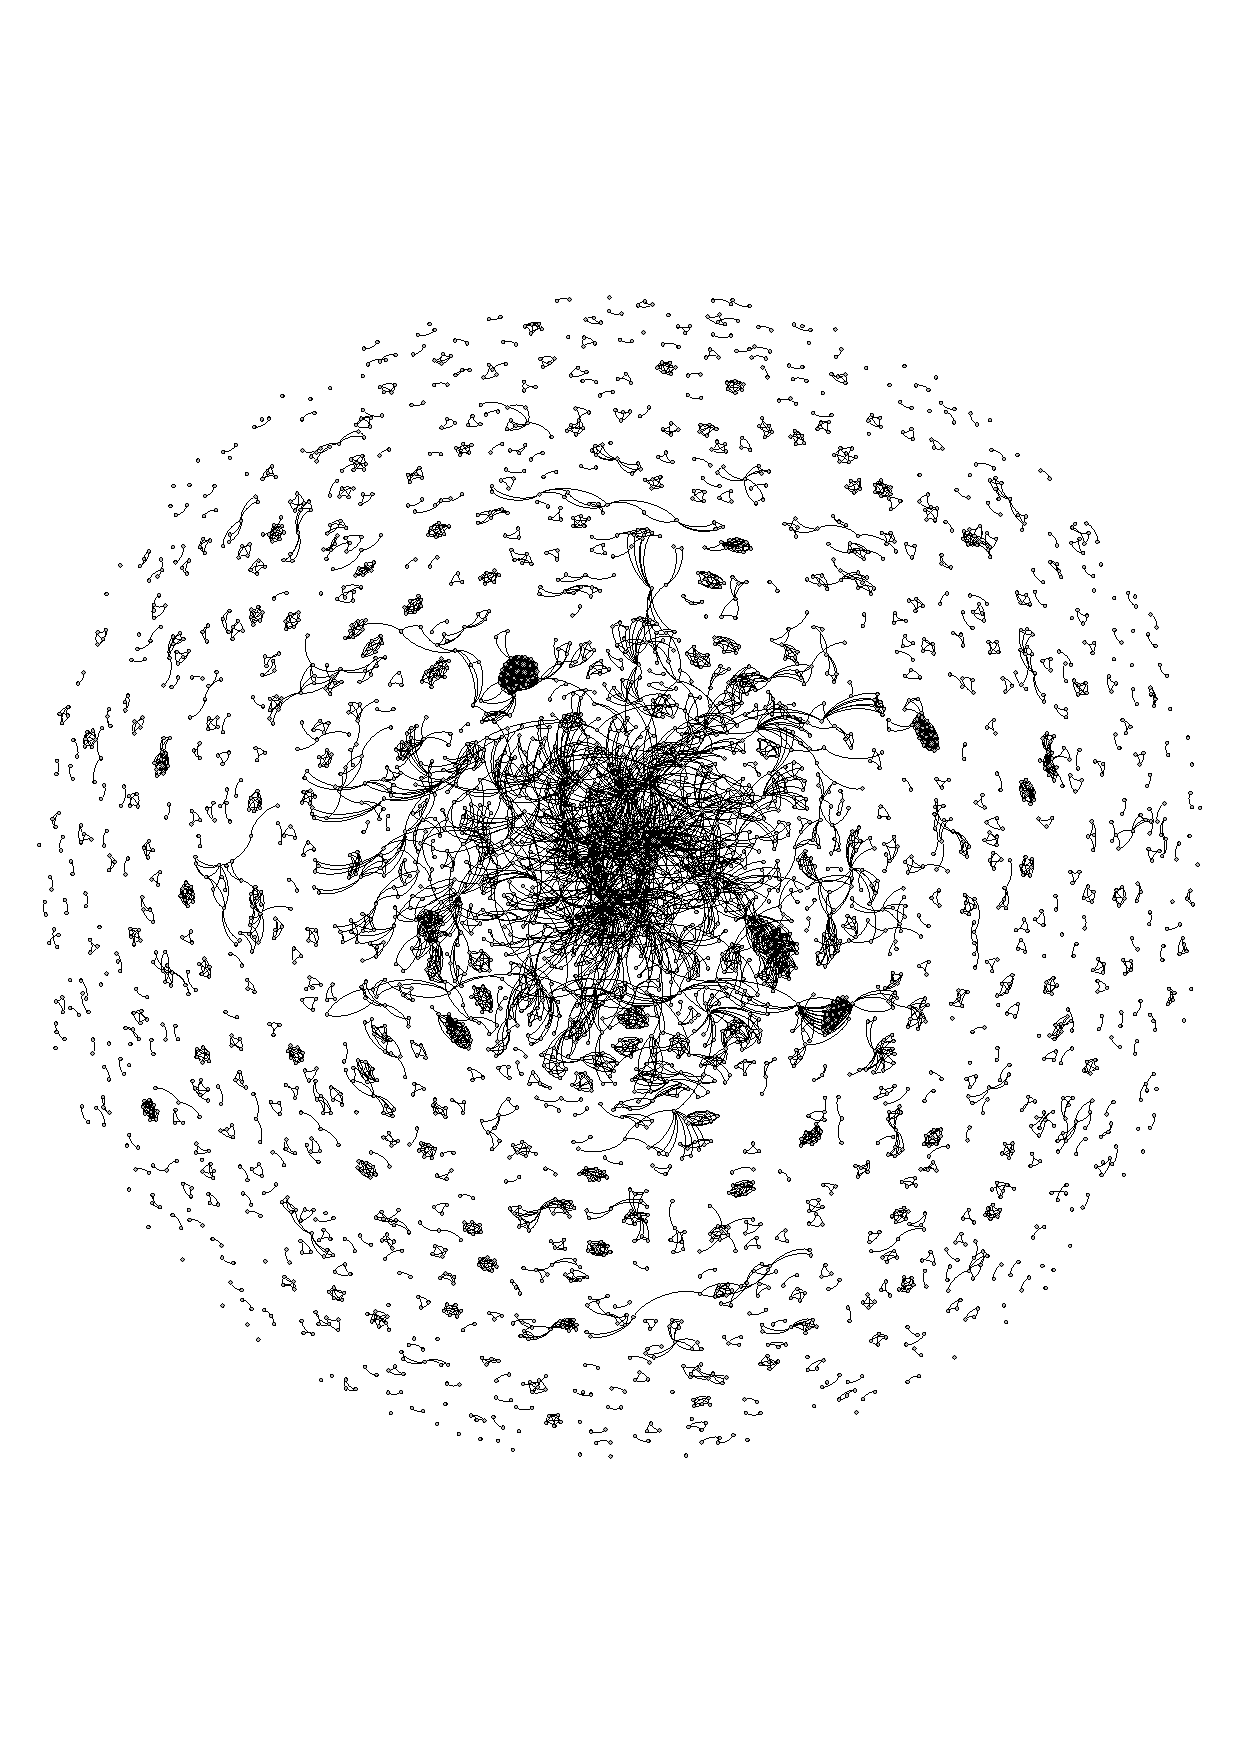
\includegraphics[width=\textwidth]{src/chapters/03/paper/bibliometric-study-of-the-prisoners-dilemma/assets/images/pd_network.pdf}
    \caption{\(G\) the co-authorship network for the IPD.}\label{fig:graphical_representation_g}
\end{figure}

\begin{figure}[!hbtp]
    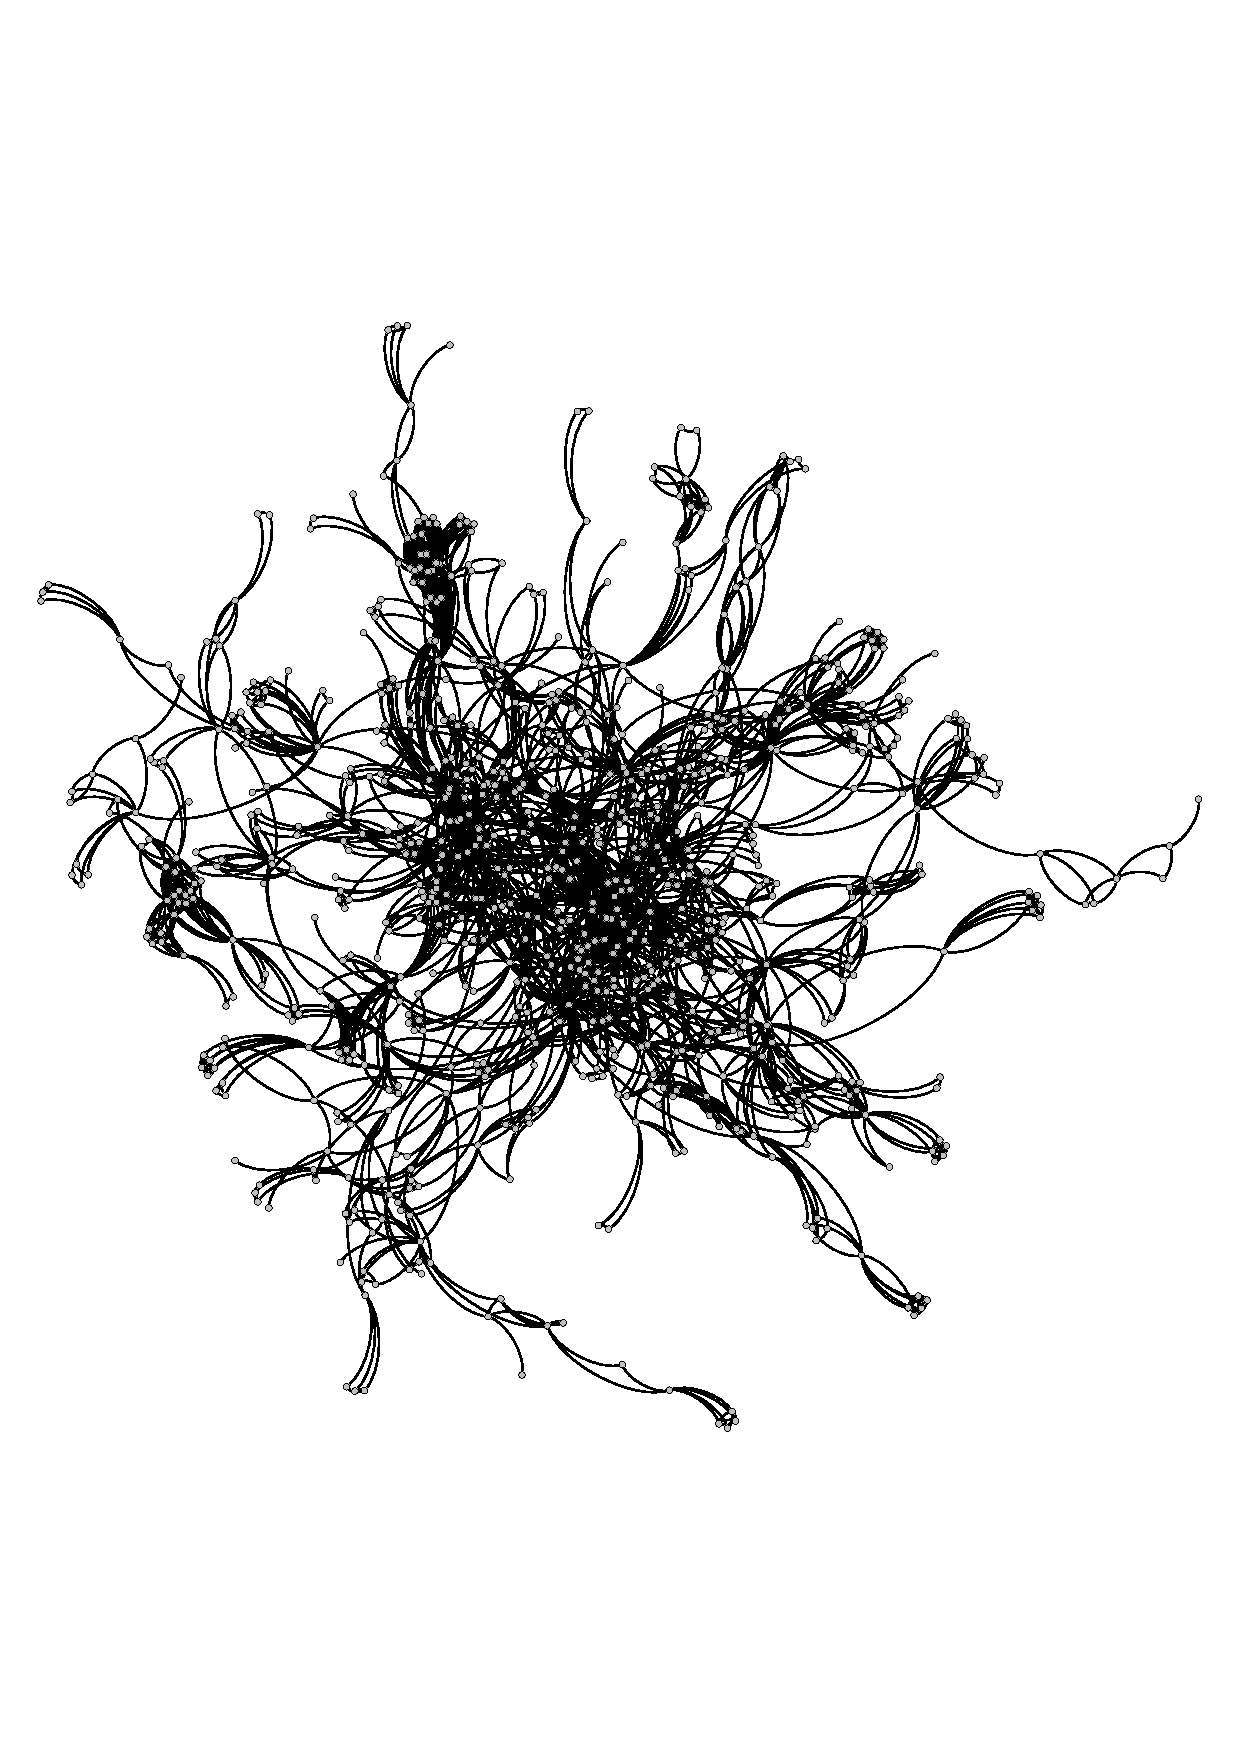
\includegraphics[width=\textwidth]{src/chapters/03/paper/bibliometric-study-of-the-prisoners-dilemma/assets/images/pd_network_cluster.pdf}
    \caption{\(\bar{G}\) the largest connected component of \(G\).}\label{fig:graphical_representation_g_bar}
\end{figure}

Based on Table~\ref{table:network_comparison.tex} an author in \(G\) has on
average 4 collaborators and a 70\% probability of collaborating with a
collaborator's co-author. An author of \(\bar{G}\) on average is 7\% more likely
to write with a collaborator's co-author and on average has 2 more
collaborators. Moreover, there are only \isolatedpercentage\% of authors in the
PD that has no connection to any other author.

\begin{table}[!hbtp]
    \centering
    \resizebox{\textwidth}{!}{
    \begin{tabular}{lrrrrrrrrrr}
\toprule
{} &  \# Nodes &  \# Edges  &  \% Isolated nodes &  \# Connected components &  Size of largest component &  Av. degree &  \# Communities &  Modularity &  Clustering coeff \\
\midrule
$G$       &     4011 &     7642 &               3.2 &                     947 &                        796 &       3.811 &            967 &     0.96491 &             0.701 \\
$\bar{G}$ &      796 &     2214 &               0.0 &                       1 &                        796 &       5.563 &             25 &     0.84406 &             0.773 \\
\bottomrule
\end{tabular}
}
    \caption{Network metrics for \(G\) and \(\bar{G}\) respectively.}
    \label{table:network_comparison.tex}
\end{table}

But how do these compare to other fields? Two more data sets for the topics
``Price of Anarchy'' and ``Auction Games'' have been collected in order to
compare the collaborative behaviour of the PD to other game theoretic fields. A
total of 3444 publications have been collected for Auction games and 748 for
Price of Anarchy. Price of Anarchy is relatively a new field, with the first
publication on the topic being~\cite{Koutsoupias1999} in 1999. This explains the
small number of articles that have been retrieved. Both data sets have been
archived and are available in~\cite{auction_data_2018, anarchy_data_2018}.
The networks for both data sets have been generated in the same way as \(G\).
A summary of the networks' metrics are given by Table~\ref{table:other_topics_network_comparison.tex}.

\begin{table}[!hbtp]
    \centering
    \resizebox{\textwidth}{!}{
    \begin{tabular}{lrrrrP{0.2\textwidth}P{0.2\textwidth}rrrrr}
\toprule
{} &  \# Nodes &  \# Edges &  \# Isolated nodes &  \% Isolated nodes &  \# Connected components &  Size of largest component &  Av. degree &  \# Communities &  Modularity &  Clustering coeff \\
\midrule
auction Games    &     5165 &     7861 &               256 &               5.0 &                    1272 &                       1348 &       3.044 &           1294 &       0.957 &             0.622 \\
price of Anarchy &     1155 &     1953 &                 4 &               0.3 &                     245 &                        222 &       3.382 &            253 &       0.965 &             0.712 \\
\bottomrule
\end{tabular}
}
    \caption{Network metrics for auction games and price of anarchy networks respectively.}
    \label{table:other_topics_network_comparison.tex}
\end{table}

The average degrees for the Price of Anarchy and for Auction games are lower
than the PD's. In Auction games an author is more likely to have no collaborators,
and in the Price of Anarchy there are almost no authors that are not connected
to someone. This could be an effect of the field being introduced in more modern
days. Overall, an author in the PD has on average more collaborators
and there are less isolated authors compared to another well established game
theoretic field. These results seem to indicate that the PD is a \textit{relatively} collaborative
field.

However, both \(G\) and \(\bar{G}\) have a high modularity (larger than 0.84) and a large number of
communities (967 and 25 respectively). A high modularity implies that authors create their own publishing
communities but not many publications from authors from different communities
occur. Thus, author tends to collaborate with authors in their communities but
not many efforts are made to create new connections to other communities and
spread the knowledge of the field across academic teams. The fields
of both Price of Anarchy and Auction games also have high modularity, and
that could indicate that is in fact how academic publications are.
Thus, the PD is indeed a collaborative field but perhaps it is not
more collaborative than other fields, as there is no effort from the authors
to write with people outside their community.

The evolution of the networks was also explored over time by constructing the
network cumulatively over 51 periods. Except from the first period 1951-1966 the
rest of the periods have a yearly interval (data for the years 1975 and 1982
were not retrieved by the collection data process). The metrics of each sub
network are given by Tables~\ref{table:cumulative_graphs} and~\ref{table:cumulative_clusters}.

\begin{table}[!hbtp]
    \centering
    \resizebox{.9\textwidth}{!}{
    \begin{tabular}{lrrrrrrrrrr}
\toprule
Period &  \# Nodes &  \# Edges &  \% Isolated nodes &  \multicolumn{1}{p{3cm}}{\centering Size of largest component} &  Av. degree &  \# Communities &  Modularity &  Clustering coeff \\
\midrule
1951 - 1966 &        2 &        1 &    0.0 &     2 &       1.000 &              1 &       0.000 &             0.000 \\
1951 - 1967 &        2 &        1 &    0.0 &     2 &       1.000 &              1 &       0.000 &             0.000 \\
1951 - 1968 &        5 &        8 &    0.0 &     5 &       3.200 &              1 &       0.000 &             0.867 \\
1951 - 2002 &        7 &       21 &    0.0 &     7 &       6.000 &              1 &       0.000 &             1.000 \\
1951 - 2003 &        7 &       21 &    0.0 &     7 &       6.000 &              1 &       0.000 &             1.000 \\
1951 - 2004 &       10 &       13 &    0.0 &    10 &       2.600 &              2 &       0.376 &             0.553 \\
1951 - 2005 &       19 &       28 &    0.0 &    19 &       2.947 &              3 &       0.544 &             0.730 \\
1951 - 2006 &       22 &       35 &    0.0 &    22 &       3.182 &              4 &       0.527 &             0.720 \\
1951 - 2007 &       25 &       39 &    0.0 &    25 &       3.120 &              5 &       0.558 &             0.686 \\
1951 - 2008 &       33 &       62 &    0.0 &    33 &       3.758 &              4 &       0.623 &             0.736 \\
1951 - 2009 &       71 &      148 &    0.0 &    71 &       4.169 &              6 &       0.697 &             0.698 \\
1951 - 2010 &      133 &      387 &    0.0 &   133 &       5.820 &              7 &       0.726 &             0.749 \\
1951 - 2011 &      157 &      465 &    0.0 &   157 &       5.924 &              8 &       0.727 &             0.725 \\
1951 - 2012 &      209 &      611 &    0.0 &   209 &       5.847 &             11 &       0.733 &             0.737 \\
1951 - 2013 &      322 &      892 &    0.0 &   322 &       5.540 &             12 &       0.780 &             0.743 \\
1951 - 2014 &      399 &     1109 &    0.0 &   399 &       5.559 &             15 &       0.794 &             0.742 \\
1951 - 2015 &      504 &     1368 &    0.0 &   504 &       5.429 &             24 &       0.811 &             0.751 \\
1951 - 2016 &      613 &     1677 &    0.0 &   613 &       5.471 &             21 &       0.819 &             0.761 \\
1951 - 2017 &      706 &     1935 &    0.0 &   706 &       5.482 &             29 &       0.830 &             0.772 \\
1951 - 2018 &      796 &     2214 &    0.0 &   796 &       5.563 &             25 &       0.845 &             0.773 \\
\bottomrule
\end{tabular}
}
    \caption{Collaborativeness metrics for cumulative graphs' main clusters, \(\tilde{G} \subseteq \bar{G}\)}\label{table:cumulative_clusters}
\end{table}

\begin{table}[!hbtp]
    \centering
    \resizebox{\textwidth}{!}{
    \begin{tabular}{lrrrrrrrrrr}
\toprule
Period &  \# Nodes &  \# Edges &  \% Isolated nodes &  \multicolumn{1}{p{3cm}}{\centering \# Connected components} &  \multicolumn{1}{p{3cm}}{\centering Size of largest component} &  Av. degree &  \# Communities &  Modularity &  Clustering coeff \\
\midrule
1951 - 1966 &        6 &        3 &    0.0 &                       3 &                          2 &       1.000 &              3 &       0.667 &             0.000 \\
1951 - 1967 &        8 &        4 &    0.0 &                       4 &                          2 &       1.000 &              4 &       0.750 &             0.000 \\
1951 - 1968 &       19 &       15 &    0.0 &                       8 &                          5 &       1.579 &              8 &       0.684 &             0.228 \\
1951 - 1969 &       20 &       17 &    0.0 &                       8 &                          6 &       1.700 &              8 &       0.630 &             0.250 \\
1951 - 1970 &       22 &       18 &    0.0 &                       9 &                          6 &       1.636 &              9 &       0.667 &             0.227 \\
1951 - 1971 &       33 &       28 &    0.0 &                      13 &                          6 &       1.697 &             13 &       0.827 &             0.424 \\
1951 - 1972 &       39 &       34 &    0.0 &                      15 &                          6 &       1.744 &             15 &       0.867 &             0.513 \\
1951 - 1973 &       42 &       35 &    2.4 &                      17 &                          6 &       1.667 &             17 &       0.873 &             0.476 \\
1951 - 1974 &       42 &       35 &    2.4 &                      17 &                          6 &       1.667 &             17 &       0.873 &             0.476 \\
1951 - 1976 &       42 &       35 &    2.4 &                      17 &                          6 &       1.667 &             17 &       0.873 &             0.476 \\
1951 - 1977 &       44 &       36 &    2.3 &                      18 &                          6 &       1.636 &             18 &       0.880 &             0.455 \\
1951 - 1978 &       44 &       36 &    2.3 &                      18 &                          6 &       1.636 &             18 &       0.880 &             0.455 \\
1951 - 1979 &       47 &       40 &    2.1 &                      18 &                          6 &       1.702 &             18 &       0.884 &             0.454 \\
1951 - 1980 &       47 &       40 &    2.1 &                      18 &                          6 &       1.702 &             18 &       0.884 &             0.454 \\
1951 - 1981 &       50 &       46 &    2.0 &                      18 &                          6 &       1.840 &             18 &       0.889 &             0.497 \\
1951 - 1983 &       51 &       46 &    3.9 &                      19 &                          6 &       1.804 &             19 &       0.889 &             0.487 \\
1951 - 1984 &       53 &       47 &    3.8 &                      20 &                          6 &       1.774 &             20 &       0.894 &             0.469 \\
1951 - 1985 &       53 &       47 &    3.8 &                      20 &                          6 &       1.774 &             20 &       0.894 &             0.469 \\
1951 - 1986 &       53 &       47 &    3.8 &                      20 &                          6 &       1.774 &             20 &       0.894 &             0.469 \\
1951 - 1987 &       56 &       48 &    5.4 &                      22 &                          6 &       1.714 &             22 &       0.898 &             0.443 \\
1951 - 1988 &       62 &       52 &    6.5 &                      25 &                          6 &       1.677 &             25 &       0.909 &             0.449 \\
1951 - 1989 &       75 &       62 &    6.7 &                      31 &                          6 &       1.653 &             31 &       0.926 &             0.424 \\
1951 - 1990 &       79 &       64 &    6.3 &                      33 &                          6 &       1.620 &             33 &       0.930 &             0.403 \\
1951 - 1991 &       87 &       69 &    6.9 &                      37 &                          6 &       1.586 &             37 &       0.937 &             0.400 \\
1951 - 1992 &       95 &       72 &   10.5 &                      42 &                          6 &       1.516 &             42 &       0.941 &             0.367 \\
1951 - 1993 &      106 &       81 &   11.3 &                      47 &                          6 &       1.528 &             47 &       0.947 &             0.366 \\
1951 - 1994 &      124 &       95 &   12.9 &                      56 &                          6 &       1.532 &             56 &       0.955 &             0.394 \\
1951 - 1995 &      135 &      102 &   12.6 &                      61 &                          6 &       1.511 &             61 &       0.960 &             0.384 \\
1951 - 1996 &      142 &      105 &   12.7 &                      65 &                          6 &       1.479 &             65 &       0.962 &             0.365 \\
1951 - 1997 &      155 &      115 &   12.9 &                      71 &                          6 &       1.484 &             71 &       0.966 &             0.392 \\
1951 - 1998 &      191 &      140 &   11.0 &                      87 &                          6 &       1.466 &             87 &       0.973 &             0.367 \\
1951 - 1999 &      221 &      169 &   11.3 &                      99 &                          6 &       1.529 &             99 &       0.977 &             0.397 \\
1951 - 2000 &      250 &      195 &   10.8 &                     110 &                          6 &       1.560 &            110 &       0.979 &             0.418 \\
1951 - 2001 &      287 &      235 &   10.5 &                     125 &                          7 &       1.638 &            125 &       0.977 &             0.419 \\
1951 - 2002 &      335 &      278 &   10.7 &                     146 &                          7 &       1.660 &            146 &       0.979 &             0.428 \\
1951 - 2003 &      381 &      310 &   10.5 &                     168 &                          7 &       1.627 &            168 &       0.982 &             0.413 \\
1951 - 2004 &      437 &      370 &    9.2 &                     185 &                         10 &       1.693 &            185 &       0.983 &             0.424 \\
1951 - 2005 &      532 &      476 &    7.7 &                     214 &                         19 &       1.789 &            214 &       0.985 &             0.458 \\
1951 - 2006 &      640 &      603 &    6.7 &                     246 &                         22 &       1.884 &            246 &       0.987 &             0.486 \\
1951 - 2007 &      793 &      877 &    5.8 &                     283 &                         25 &       2.212 &            283 &       0.985 &             0.532 \\
1951 - 2008 &      948 &     1170 &    5.3 &                     318 &                         33 &       2.468 &            319 &       0.985 &             0.558 \\
1951 - 2009 &     1108 &     1442 &    4.9 &                     356 &                         71 &       2.603 &            358 &       0.982 &             0.573 \\
1951 - 2010 &     1300 &     1936 &    5.1 &                     402 &                        133 &       2.978 &            405 &       0.965 &             0.592 \\
1951 - 2011 &     1560 &     2375 &    5.1 &                     472 &                        157 &       3.045 &            475 &       0.970 &             0.613 \\
1951 - 2012 &     1837 &     2865 &    4.4 &                     534 &                        209 &       3.119 &            537 &       0.969 &             0.634 \\
1951 - 2013 &     2149 &     3420 &    4.3 &                     603 &                        322 &       3.183 &            609 &       0.965 &             0.644 \\
1951 - 2014 &     2481 &     3971 &    4.2 &                     683 &                        399 &       3.201 &            694 &       0.962 &             0.658 \\
1951 - 2015 &     2938 &     4877 &    3.7 &                     765 &                        504 &       3.320 &            779 &       0.965 &             0.675 \\
1951 - 2016 &     3469 &     6532 &    3.3 &                     850 &                        613 &       3.766 &            863 &       0.964 &             0.696 \\
1951 - 2017 &     3735 &     7072 &    3.2 &                     895 &                        706 &       3.787 &            912 &       0.964 &             0.700 \\
1951 - 2018 &     4011 &     7642 &    3.2 &                     947 &                        796 &       3.811 &            967 &       0.966 &             0.701 \\
\bottomrule
\end{tabular}
}
    \caption{Collaborativeness metrics for cumulative graphs, \(\tilde{G} \subseteq G\)}\label{table:cumulative_graphs}
\end{table}

The results, similarly to the results of~\cite{Liu2015}, confirm that the
networks grow over time and that the networks always had a high modularity.
Since the first publications authors tend to write with people from their
communities, and that is not an effect of a specific time period.

The networks corresponding to the topics of Section~\ref{section:preliminary} have
also been generated similarly to \(G\). Note that authors with publications in
more than one topic exist, and these authors are included in all the corresponding
networks. A metrics' summary for all five topic networks is given by Table
\ref{table:topics_networks}.

\begin{table}[!hbtp]
    \centering
    \resizebox{\textwidth}{!}{
    \begin{tabular}{lrrrrrrrrrr}
\toprule
{} &  \# Nodes &  \# Edges &  \# Isolated nodes &  \% Isolated nodes &  \# Connected components &  Size of largest component &  Av. degree &  \# Communities &  Modularity &  Clustering coeff \\
\midrule
Topic A &     1124 &     2137 &                15 &               1.3 &                     264 &                         56 &       3.802 &            265 &       0.983 &             0.759 \\
Topic B &      695 &     1382 &                13 &               1.9 &                     157 &                         80 &       3.977 &            158 &       0.950 &             0.773 \\
Topic C &      900 &     1141 &                41 &               4.6 &                     281 &                         29 &       2.536 &            281 &       0.981 &             0.636 \\
Topic D &      880 &     1509 &                17 &               1.9 &                     174 &                        312 &       3.430 &            183 &       0.918 &             0.701 \\
Topic E &     1045 &     1964 &                59 &               5.6 &                     354 &                         31 &       3.759 &            354 &       0.926 &             0.664 \\
\bottomrule
\end{tabular}
}
    \caption{Network metrics for topic networks.}\label{table:topics_networks}
\end{table}

Topic B is the network with the highest average degree followed by Topic A. The
topic with the smallest average degree, 2.5, is Topic C. In topics A and B the
number of isolated nodes is very small \(less than (0.2)\) compared to Topic E where the
percentage of isolated nodes is approximately 6\%. Moreover, in topics C and E
an author is 10\% more likely to collaborate with a collaborator's co-author.
Thus, topics ``human subject research'' and ``biological studies'' tend
to be more collaborative than the topic of ``strategies'', and an authors in
these are less likely to have at least one collaborator compared to the topic of
``modelling problems as a PD''.

``Evolutionary dynamics on networks'' also appear to be a collaborative topic.
In fact the network of the topic  is a
sub graph of \(\bar{G}\), the main cluster of \(G\) and it will be demonstrated in the following section that
authors in this network are more like to gain from the influence of the network
compared to any other topic network.

The two centrality measures reported in this thesis are closeness and
betweenness centrality. Closeness centrality is a measure of how easy it is for
an author to contact others, and consequently affect them; influence them. Thus
closeness centrality is a measure of influence. Betweenness centrality is a
measure of how many paths pass through a specific node, thus the amount of
information this person has access to. Betweenness centrality is interpreted as a
measure of how much an author gains from the field. The values of the centralities
can range between 0 and 1. Influence and the amount of information
an author has access to are proxies to understand if/which authors benefit more
from their position.

For \(G\) and \(\bar{G}\) the most central authors based on closeness and
betweenness centralities are given by Table~\ref{table:central_authors}. The
most central authors in \(G\) and \(\bar{G}\) are the same. This implies that
the results on centrality heavily rely on the main cluster (as expected). Matjaz Perc is an
author with 83 publications in the data set and the most central authors based
on both centrality measures. The most central authors are fairly similar between
the two measures. The author that appear to be central based on one measure and
not the other are Martin Nowak, Franz Weissing, Jianye Hao, Angel Sanchez and
Valerio Capraro which have access to information due to their
positioning but do not influence the network as much, and the opposite is true
for Attila Szolnoki, Luo-Luo Jiang Sandro Meloni, Cheng-Yi Xia and Xiaojie Chen.

\begin{table}[!hbtp]
    \begin{center}
    \resizebox{.9\textwidth}{!}{\begin{tabular}{lgrgr|grgr}
\toprule
& \multicolumn{4}{c}{$G$} & \multicolumn{4}{c}{$\bar{G}$} \\
\midrule
{} &             Name &  Betweenness &             Name &  Closeness &             Name &  Betweenness &             Name &  Closeness \\
\midrule
1  &      Matjaz Perc &        0.015 &      Matjaz Perc &      0.066 &      Matjaz Perc &        0.373 &      Matjaz Perc &      0.330 \\
2  &        Zhen Wang &        0.011 &        Long Wang &      0.060 &        Zhen Wang &        0.279 &        Long Wang &      0.301 \\
3  &        Long Wang &        0.007 &     Yamir Moreno &      0.059 &        Long Wang &        0.170 &     Yamir Moreno &      0.299 \\
4  &     Martin Nowak &        0.006 &  Attila Szolnoki &      0.059 &     Martin Nowak &        0.159 &  Attila Szolnoki &      0.297 \\
5  &    Angel Sanchez &        0.004 &        Zhen Wang &      0.059 &    Angel Sanchez &        0.114 &        Zhen Wang &      0.296 \\
6  &     Yamir Moreno &        0.004 &    Arne Traulsen &      0.056 &     Yamir Moreno &        0.110 &    Arne Traulsen &      0.281 \\
7  &    Arne Traulsen &        0.004 &    Luo-Luo Jiang &      0.055 &    Arne Traulsen &        0.107 &    Luo-Luo Jiang &      0.280 \\
8  &   Franz Weissing &        0.004 &    Sandro Meloni &      0.055 &   Franz Weissing &        0.101 &    Sandro Meloni &      0.278 \\
9  &       Jianye Hao &        0.004 &     Cheng-Yi Xia &      0.055 &       Jianye Hao &        0.094 &     Cheng-Yi Xia &      0.276 \\
10 &  Valerio Capraro &        0.004 &     Xiaojie Chen &      0.055 &  Valerio Capraro &        0.093 &     Xiaojie Chen &      0.276 \\
\bottomrule
\end{tabular}
}
\end{center}
\caption{10 most central authors based on betweenness and closeness centralities
for \(G\) and \(\bar{G}\).}\label{table:central_authors}
\end{table}

It is obvious that in \(G\) the centrality values are low which suggests
that in the PD authors do not benefit from their positions. This could be an
effect of information not flowing from one community to another as authors tend
to write with people from their communities. Nevertheless,
there are authors that do benefit from their position, but these are
only the authors connected to the main cluster.

The centrality measures for the topic networks have also been estimated and are
given in
Tables~\ref{table:central_authors_bc_topics}-\ref{table:central_authors_cc_topics}.
If information was flowing between the communities of the research topics then
there would be an increase to the values of centralities for the sub networks.
However, the only topic where authors gain from their positions are the authors
of Topic D (topic on evolutionary dynamics on network). From the list of names it is obvious that these authors are
part of \(\bar{G}\), and that the network of Topic D is a sub network of \(\bar{G}\).
This confirms the results. The people benefiting from their position in the co-authorship networks
corresponding to research topics of the PD are only the people from the main
cluster of \(G\).

\newcolumntype{g}{>{\columncolor{Gray}}l}
\begin{table}[!hbtp]
    \begin{center}
    \resizebox{.9\textwidth}{!}{\begin{tabular}{lggllggllgg}
\toprule
& \multicolumn{2}{g}{Topic A} & \multicolumn{2}{c}{Topic B} & \multicolumn{2}{g}{Topic C} & \multicolumn{2}{c}{Topic D} & \multicolumn{2}{g}{Topic E}\\
\midrule
{} &                 Name &  Betweeness &             Name &  Betweeness &             Name &  Betweeness &              Name &  Betweeness &                  Name &  Betweeness \\
\midrule
1  &           David Rand &       0.002 &        Long Wang &       0.006 &   Daniel Ashlock &       0.001 &       Matjaz Perc &       0.064 &             Zengru Di &         0.0 \\
2  &      Valerio Capraro &       0.001 &    Luo-Luo Jiang &       0.005 &      Matjaz Perc &       0.000 &     Luo-Luo Jiang &       0.037 &             Jian Yang &         0.0 \\
3  &        Angel Sanchez &       0.001 &     Martin Nowak &       0.004 &       Karl Tuyls &       0.000 &      Yamir Moreno &       0.031 &  Yevgeniy Vorobeychik &         0.0 \\
4  &              Feng Fu &       0.001 &      Matjaz Perc &       0.003 &  Philip Hingston &       0.000 &  Christoph Hauert &       0.027 &       Otavio Teixeira &         0.0 \\
5  &         Martin Nowak &       0.000 &  Attila Szolnoki &       0.003 &     Eun-Youn Kim &       0.000 &         Long Wang &       0.024 &      Roberto Oliveira &         0.0 \\
6  &  Nicholas Christakis &       0.000 &  Christian Hilbe &       0.002 &    Wendy Ashlock &       0.000 &         Zhen Wang &       0.024 &              M. Nowak &         0.0 \\
7  &   Pablo Branas-Garza &       0.000 &     Yamir Moreno &       0.002 &  Attila Szolnoki &       0.000 &      Han-Xin Yang &       0.023 &             M. Harper &         0.0 \\
8  &     Toshio Yamagishi &       0.000 &     Xiaojie Chen &       0.002 &       Seung Baek &       0.000 &      Martin Nowak &       0.020 &              Xiao Han &         0.0 \\
9  &         James Fowler &       0.000 &    Arne Traulsen &       0.002 &     Martin Nowak &       0.000 &     Angel Sanchez &       0.017 &            Zhesi Shen &         0.0 \\
10 &            Long Wang &       0.000 &        Zhen Wang &       0.002 &    Thore Graepel &       0.000 &       Zhihai Rong &       0.016 &           Wen-Xu Wang &         0.0 \\
\bottomrule
\end{tabular}
}
\end{center}
\caption{10 most central authors based on betweenness centrality
for topics' networks.}\label{table:central_authors_bc_topics}
\end{table}

\newcolumntype{g}{>{\columncolor{Gray}}l}
\begin{table}[!hbtp]
    \begin{center}
    \resizebox{.9\textwidth}{!}{\begin{tabular}{lggllggllgg}
\toprule
& \multicolumn{2}{g}{Topic A} & \multicolumn{2}{c}{Topic B} & \multicolumn{2}{g}{Topic C} & \multicolumn{2}{c}{Topic D} & \multicolumn{2}{g}{Topic E}\\
\midrule
{} &                 Name &  Closeness &               Name &  Closeness &                 Name &  Closeness &             Name &  Closeness &             Name &  Closeness \\
\midrule
1  &           David Rand &      0.027 &          Long Wang &      0.043 &           Karl Tuyls &      0.022 &      Matjaz Perc &      0.123 &  Stefanie Widder &      0.029 \\
2  &      Valerio Capraro &      0.023 &        Matjaz Perc &      0.041 &        Thore Graepel &      0.019 &        Zhen Wang &      0.109 &   Rosalind Allen &      0.029 \\
3  &       Jillian Jordan &      0.022 &    Attila Szolnoki &      0.040 &           Joel Leibo &      0.018 &        Long Wang &      0.107 &  Thomas Pfeiffer &      0.029 \\
4  &  Nicholas Christakis &      0.021 &       Martin Nowak &      0.040 &        Edward Hughes &      0.017 &     Yamir Moreno &      0.105 &    Thomas Curtis &      0.029 \\
5  &         James Fowler &      0.020 &  Olivier Tenaillon &      0.038 &     Matthew Phillips &      0.017 &    Luo-Luo Jiang &      0.104 &     Carsten Wiuf &      0.029 \\
6  &         Martin Nowak &      0.020 &       Xiaojie Chen &      0.038 &  Edgar Duenez-Guzman &      0.017 &  Attila Szolnoki &      0.103 &    William Sloan &      0.029 \\
7  &        Angel Sanchez &      0.019 &             Bin Wu &      0.038 &    Antonio Castaneda &      0.017 &     Gyorgy Szabo &      0.102 &     Otto Cordero &      0.029 \\
8  &    Gordon Kraft-Todd &      0.019 &      Yanling Zhang &      0.037 &         Iain Dunning &      0.017 &     Xiaojie Chen &      0.102 &        Sam Brown &      0.029 \\
9  &        Akihiro Nishi &      0.019 &            Feng Fu &      0.037 &             Tina Zhu &      0.017 &    Guangming Xie &      0.101 &     Babak Momeni &      0.029 \\
10 &        Anthony Evans &      0.019 &         David Rand &      0.037 &          Kevin Mckee &      0.017 &     Lucas Wardil &      0.101 &     Wenying Shou &      0.029 \\
\bottomrule
\end{tabular}
}
\end{center}
\caption{10 most central authors based on closeness centrality
for topics' networks.}\label{table:central_authors_cc_topics}
\end{table}

The fact that most authors of the main cluster are primarily publishing in
evolutionary dynamics on networks indicates that publishing in this specific
topic differs from the other topics covered in this manuscript. There appears to
be more collaboration and influence in the publications on evolutionary
dynamics and authors are more likely to gain from their position,
though it is not clear as to why.

The distributions of both centrality measures for all the networks of this
work are given in the Appendix~\ref{appendix:distributions}.

\section{Chapter summary}\label{section:conclusion}

This Chapter explored the research topics from a collection of \totalarticles publications of the
Iterated Prisoner's Dilemma, and moreover, the authors' collaborative behaviour
and their influence in the research field. This was achieved by
applying network theoretic approaches and a LDA algorithm to the collection of publications.
Both the software~\cite{nikoleta_2017} and the main data set associated with the Chapter~\cite{nikoleta_2017}
have been archived and are available to be used by other researchers. In
fact Arcas has been used by~\cite{brane} and~\cite{arcas_blog}.

Arcas, it's development and the data collection were covered in section~\ref{section:methodology},
as well as an introduction to the co-authorship network and to LDA.
section~\ref{section:preliminary} covered an initial analysis of the data set
which demonstrated that the PD is a field that continues to attract academic
attention and publications. In Section~\ref{section:topics} LDA was
applied to the data set to identify topics on which researchers have been
publishing. The LDA analysis showed that the data could be classified into 5
topics associated with human subject research, biological studies, strategies,
evolutionary dynamics on networks and modelling
problems as a PD. These topics summarize the field of the PD well, as they
demonstrate its interdisciplinarity and applications to a variety of problems. A
temporal analysis explored how relevant these topics have been over the course
of time, and it revealed that even though there were not the necessarily always
the most discussed topics they were still being explored by researchers.

The collaborative behaviour of the field was explored in
section~\ref{section:co_authorship} by constructing the co-authorship network.
It was concluded that the field is a collaborative field, where authors are
likely to write with a collaborator's co-authors and on average an author has 4
co-authors, however it not necessarily more collaborative than other fields. The
authors tend to collaborate with authors from one community, but not many
authors are involved in multiple communities. This however
might be an effect of academic research, and it might not be true just for the
field of the PD. Exploring the influence of authors and their gain from being in
the network of the field demonstrated that authors do not gain much, and the
authors with influence are only the ones connected to the main cluster, to a
``main'' group of authors. This `main'' group of authors consists of authors
publishing in evolutionary dynamics on networks. Thus, an author would be aiming
to publish on this topic if they were interested in gaining from their position
in the publications of the PD.

The study of the PD is the study of cooperation and investigating the
cooperative behaviours of authors is what this Chapter has aimed to achieve. The
following Chapters focus on best responses in changing environments of the PD,
and more specifically Chapter~\ref{chapter:meta_tournaments} studies best
responses from a collection of strategies in a large number of IPD tournaments.
